\section{Finding The Best Approximation}
\label{sec:search}

Our problem may be solved na\"{\i}vely by an exhaustive search over the possible refinements. However, the search space of refinements becomes intractably large even with relatively modest datasets, as the number of possible refinements is exponential in the number of the query's attributes.
% the sum of $\domain(\pi_A(D))$ for every categorical attribute $A$ with a predicate over it.
%\felix{was shown in \cite{LMSJ23} where the number of possible refinements is bounded by $$\mathcal{O} \left( \Pi_{(A \diamond C) \in \num(Q)} |\domain(\pi_A(D))| \cdot 2^{\sum_{(\bigvee_{c \in C} A = c) \in \cat(Q)} \domain(\pi_A(D)} \right)$$}. 
Beyond the high cost of an exhaustive search, a na\"{\i}ve solution would require the evaluation of each refinement query on the DBMS to check its deviation from the constraint set. 

To address these challenges, we propose a solution based on a mixed-integer linear program (MILP). Mixed-integer linear programming is a model for optimizing a linear objective function subject to a set of expressions (equalities and inequalities) linear in the discrete or continuous variables of the problem, limiting the space of feasible assignments. Solvers for such programs have been developed with techniques to solve even large problems efficiently in practice, as discussed in \cite{QFix}.
%\yuval{is tractable a correct term here? I believe the problems are still hard but can be solved efficiently in practice}
By incorporating the concepts introduced in~\cite{MLJ22, ERICA}, we utilize data annotations to depict potential refinements. These annotations serve as variables in the MILP, and enable us to quantify the deviation from the constraint set without having to reevaluate refinements across the DBMS.

Briefly, a solution for a MILP is an assignment for the variables in the expressions, such that they are satisfied and the objective function is minimized. 
Intuitively, given a database $D$, a query $Q$, a constraint set $\constraints$, a maximum deviation from the constraint set $0 \leq \varepsilon$, and a distance measure $DIS$, we construct an instance of MILP such that the solution corresponds to a minimal refinement that produces a ranking such that its deviation is within the maximum deviation $\varepsilon$ from the constraint set $\constraints$ while minimizing $DIS$.
By formulating \problem{} as a MILP, we can leverage existing tools to streamline the search process. 


It is important to note that by using MILP to represent the problem, we are limited to distance measures that can be modeled by a linear program. However, this limitation still allows a wide range of useful distance measures, including the ones defined in~\Cref{sec:distance}. Some of these measures may require additional modeling techniques to become linearized. For example, when modeling the Jaccard distance, we can use the Charnes-Cooper transformation~\cite{CC62}. Similarly, we can introduce auxiliary binary variables to model the version of Kendall's $\tau$ for top-$k$ lists introduced in \cite{FKS03}. %\julia{Maybe this is a better place to say what you do for Fagin's version of Kendall's tau.} \felix{$\leftarrow$ check 15/10}

\begin{table}[t!]
    \centering
    \caption{Summary of variables used in our MILP model}
    %\vspace{-0.5cm}
    \footnotesize
    \begin{tabularx}{0.48\textwidth}{c|c|X}
    {\bf Var.} & \revc{{\bf Domain}} & {\bf Description} \\
    \hline
    %  $C_{A, v}$        & Whether $v$ is included in $C$ for a cat. predicate on $A$                              \\
    $C_{A,\diamond}$  & \revc{$\mathbb{R}$} & Refined $C$ for a num. predicate on $A$ with operator $\diamond$                     \\
    $A_v$             & \revc{$\{0, 1\}$} & Whether a value $v$ is selected by the cat. predicate on $A$                           \\
    $A_{v, \diamond}$ & \revc{$\{0, 1\}$} &  Whether a value $v$ is in the range of the num. predicate on $A$ with operator $\diamond$ \\
    $r_t$            & \revc{$\{0, 1\}$} & Whether tuple $t$ is selected by the refinement                                     \\
    $s_{t}$          & \revc{$\mathbb{R}$} & Rank of tuple $t$ in the ranking generated by the refinement                              \\
    $l_{t, k}$       & \revc{$\{0, 1\}$} & Whether tuple $t$ is present in the top-$k$ of the ranking generated by the refinement          \\
    $E_{G, k}$       & \revc{$\mathbb{R}$} & Number of tuples to add (remove) to satisfy lower-bound (upper-bound) cardinality constraint    
    \end{tabularx}
    % \vspace{-1cm}
    %\yuval{TODO: update}
    \label{tab:variables}
\end{table}

The MILP instance we construct consists of two main groups of expressions: those that require that all tuples selected by the refinement are in the ranking according to the {\tt ORDER BY} expression of $Q$, and those that enforce that the derived ranking's deviation from the constraint set does not exceed the input bound $\varepsilon$. We next explain the construction of the expressions in each set\revc{, and, in order to give a more intuitive picture of the process, demonstrate in \Cref{fig:example_summary} how variables are generated from a running example and how they are combined by these expressions.}


\subsection{Modeling refinements output using expressions}

Inspired by the use of provenance for query refinements~\cite{MLJ22,ERICA}, we utilize the notion of data annotations to model refinements through a set of expressions. This set is divided into two parts. The first part is used to model the tuples that satisfy the refinement query's predicate, while the second part ensures that the selected tuples are ordered correctly by the {\tt ORDER BY} expression of the input query. We start by describing the variables used in the expressions.



% \begin{table}[ht]
%         \centering
		
% 		\label{tab:joined}
%         \hspace*{-0.5cm}
%         \footnotesize
% 		\begin{tabular}{crccrrcc}
% 		\cline{2-8}
% 		& \textbf{ID} & \textbf{Gender} & \textbf{Income} & \textbf{GPA} & \textbf{SAT $\downarrow$} & \textbf{Activity} & $\prov(t)$ \\ \cline{2-8}
% 		$i_1$ & 1           & M               & Medium         & 3.7      & 1590  & SO & $\{Activity_{SO}, GPA_{3.7}\}$\\    
% 		$i_2$ & 2           & F               & Low         & 3.8      & 1580 & SO & $\{Activity_{SO}, GPA_{3.8}\}$\\    
% 		$i_3$ & 3           & F               & Low         & 3.6      & 1560  & GD & $\{Activity_{GD}, GPA_{3.6}\}$\\    
% 		$i_4$ & 4           & M               & High         & 3.8      & 1570 & RB & $\{Activity_{RB}, GPA_{3.8}\}$\\
%         $i_4'$ & 4           & M               & High         & 3.8      & 1570 & TU & $\{Activity_{TU}, GPA_{3.8}\}$\\
% 		$i_5$ & 5           & F               & Medium         & 3.6      & 1550 & MO & $\{Activity_{MO}, GPA_{3.6}\}$\\    
% 		$i_6$ & 6           & F               & Low         & 3.7      & 1550 & SO & $\{Activity_{SO}, GPA_{3.7}\}$ \\    
% 		$i_7$ & 7           & M               & Low         & 3.7      & 1540 & RB & $\{Activity_{RB}, GPA_{3.7}\}$ \\    
% 		$i_8$ & 8           & F               & High         & 3.9      & 1530 & RB & $\{Activity_{RB}, GPA_{3.9}\}$\\
%         $i_{8}'$ & 8           & F               & High         & 3.9      & 1530 & TU & $\{Activity_{TU}, GPA_{3.9}\}$\\
% 		$i_{10}$ & 10           & M               & High         & 3.7      & 1520 & RB & $\{Activity_{RB}, GPA_{3.7}\}$\\    
% 		$i_{11}$ & 11           & F               & Low         & 3.8      & 1490 & RB & $\{Activity_{RB}, GPA_{3.8}\}$\\    
% 		$i_{12}$ & 12           & M               & Medium         & 4.0      & 1480 & RB & $\{Activity_{RB}, GPA_{4.0}\}$\\    
%   		$i_{14}$ & 14           & F               & Low         & 3.7      & 1410 & RB & $\{Activity_{RB}, GPA_{3.7}\}$\\  
% 		\end{tabular}
%   \caption{$\widetilde{Q}$ obtained from \running{}}
% \end{table}

\begin{table}%[ht]
        \centering	
  \caption{$\widetilde{Q}$ obtained from \running{}}
  \hspace*{-1cm}
        \footnotesize
		\begin{tabular}{clccc}
		\cline{2-5}
		& \textbf{ID} & \textbf{Gender} & \textbf{Income} &  $\prov(t)$ \\ \cline{2-5}
		 & $t_1$           & M               & Medium         & $\{Activity_{SO}, GPA_{3.7}\}$\\    
		 & $t_2$           & F               & Low         & $\{Activity_{SO}, GPA_{3.8}\}$\\    
		 & $t_3$           & F               & Low        & $\{Activity_{GD}, GPA_{3.6}\}$\\    
		& $t_4$            & M               & High     & $\{Activity_{RB}, GPA_{3.8}\}$\\
         & $t_4'$           & M               & High & $\{Activity_{TU}, GPA_{3.8}\}$\\
		 & $t_5$           & F               & Medium   & $\{Activity_{MO}, GPA_{3.6}\}$\\    
		& $t_6$            & F               & Low       & $\{Activity_{SO}, GPA_{3.7}\}$ \\    
		 & $t_7$           & M               & Low       & $\{Activity_{RB}, GPA_{3.7}\}$ \\    
		 & $t_8$           & F               & High      & $\{Activity_{RB}, GPA_{3.9}\}$\\
         & $t_{8}'$           & F               & High       & $\{Activity_{TU}, GPA_{3.9}\}$\\
		 & $t_{10}$           & M               & High  & $\{Activity_{RB}, GPA_{3.7}\}$\\    
		 & $t_{11}$           & F               & Low    & $\{Activity_{RB}, GPA_{3.8}\}$\\    
		 & $t_{12}$           & M               & Medium    & $\{Activity_{RB}, GPA_{4.0}\}$\\    
  	 &  $t_{14}$            & F               & Low       & $\{Activity_{RB}, GPA_{3.7}\}$\\ \cline{2-5} 
		\end{tabular}
 % \vspace{-0.5cm}
  \label{tab:joined}
\end{table}

\paragraph*{Variables} Given a query $Q$ and a dataset $D$, for each categorical predicate in $\cat(Q)$ over an attribute $A$, we define a variable $A_{v} \in \{0, 1\}$ for each value $v$ in the domain of $A$ in the $D$. Intuitively, a solution to the MILP where $A_{v} = 1$ corresponds to a refinement that includes $A = v$ in the categorical predicates. For each numerical predicate $A \diamond C \in \num(Q)$, we define a variable $C_{A, \diamond}$ \revc{whose value is in the range of values of $A$ in $D$}, and a set of variables $A_{v, \diamond}$ for each value $v$ in the domain of $A$ in $D$.

\begin{example}
% Consider again our running  example. 
$Activity_{RB}$ and $Activity_{SO}$ are \revc{two of the variables generated by the categorical predicate {\tt Activity = `RB'}
% as this predicate may be refined to include e.g. `RB' and/or `SO' 
since these values are present in the database.} 
The variable $C_{GPA, \geq}$ is generated from the numerical predicate {\tt GPA >= 3.7}. Additionally, the variable $GPA_{3.7, \geq}$ is generated since there exists a tuple in the data with the value $3.7$ in the {\tt GPA} attribute. 
\end{example} 

The value of $C_{A, \diamond}$ represents the value of the constant $C$ in the refinement query, and the variables $A_{v, \diamond}$ are used to determine whether a given tuple $t$ in $D$ (with the value $v$ in $A$) satisfies that predicate over $A$ in the refined query. More concretely, the variable $A_{v, \diamond}$ is used to reflect whether  $v \diamond C_{A, \diamond}$. Finally, we use a variable $r_t$ to denote the existence of a tuple $t$ in the output of a refinement query and a variable $s_t$ to indicate the position of $t$ in the output.

% note: we now work directly with A_{v, \diamond} variables now without the intermediate variable (saving dom(A) binary variables)
%and $A_v\in \{0, 1\}$ correspond to the satisfaction of the value $v$ in attribute $A$ of the predicates over $A$ in the query. Note that there may be two predicates over an attribute $A$ (upper bound and lower bound over the value of $A$). Thus, it is possible that $A_v\neq A_{v, \diamond}$.

% and the variables $A_v\in \{0, 1\}$, and  are used to determine whether a given tuple $t$ in $D$ (with the value $v$ in $A$) satisfies the predicate over $A$ in the refined query.

\paragraph*{Expressions}  We formulate a set of expressions such that the assignment generated by a solver to the MILP instance corresponds to the set of tuples selected by the corresponding refinement query. A tuple is part of a query's output if it satisfies its predicates set. We first define expressions for numerical predicates. Intuitively, a tuple $t$ with value $v$ in attribute $A$ satisfies the predicate $A \diamond C_{A, \diamond}$ if $v \diamond C_{A, \diamond}$. For lower-bound predicates, i.e., when $A \geq C$ or $A > C$, we model this using the following MILP expressions for each predicate in $\num(Q)$ and each value $V$ in the domain of $A$ in $D$.%$v \in \domain(\pi_A(D))$:
\begin{align}
\begin{split}
C_{A, \diamond} + M_A \cdot A_{v, \diamond} &\geq v + (1 - {\sf St}(\diamond)) \cdot \delta \label{eq:value_bounds_inline}\\
C_{A, \diamond} - M_A \cdot (1 - A_{v, \diamond}) &\leq v - {\sf St}(\diamond) \cdot \delta
\end{split}
\end{align} 
%\yuval{why not simply $v+\delta$ in the first expression?}
% \felix{more explanation?}
where $M_A$ is a constant larger than the maximum \revc{absolute} value in the domain of the attribute $A$ in $D$, ${\sf St}(\diamond)$ is $1$ if $\diamond$ is a strict inequality and $0$ otherwise, and $\delta$ is some small constant added when $\diamond$ is strict in order to relax the inequality as MILP expressions do not support strict inequalities. We choose $\delta$ to be smaller than the smallest pairwise difference between the values in the domain of $A$, ensuring the relaxation does not include another value from the domain. For upper-bound predicates, we instead use the following set of expressions.
\begin{align}
\begin{split}
C_{A, \diamond} - M_A \cdot A_{v, \diamond} &\leq v - (1 - {\sf St}(\diamond)) \cdot \delta \label{eq:value_bounds_inline2}\\
C_{A, \diamond} + M_A \cdot (1 - A_{v, \diamond}) &\geq v + {\sf St}(\diamond) \cdot \delta
\end{split}
\end{align}
 Intuitively, the first expressions in (\ref{eq:value_bounds_inline}) and (\ref{eq:value_bounds_inline2}) ensure that $A_{v, \diamond}$ is $1$ if $v \diamond C_{A, \diamond}$ is true and the second expressions are used to ensure that $A_{v, \diamond}$ is 0 if $v \diamond C_{A, \diamond}$ is false. Together, they enforce that $A_{v, \diamond}$ is $1$ if and only if $v \diamond C_{A, \diamond}$ is true.
%In the first inequalities in (\ref{eq:value_bounds_inline}) and (\ref{eq:value_bounds_inline2}), when $C_{A, \diamond}$ has a value such that $v \diamond C_{A, \diamond}$, then the only feasible assignment to $A_{v, \diamond}$ is 1. If $M_A$ is insufficiently large, then it is possible that a value of $C_{A, v}$ that makes $v \diamond C_{A, \diamond}$ true would make the inequality infeasible as adding (subtracting) $M_A$ to such a value of $C_{A, \diamond}$ would not be at least (at most) the value $v$ plus (minus) any constants needed to relax strict equalities. However, when $v \diamond C_{A, \diamond}$ is not true, these inequalities are still feasible with $A_{v, \diamond}$ being 1. Therefore, we include the second inequalities in (\ref{eq:value_bounds_inline}) and (\ref{eq:value_bounds_inline2}), for which when $v \diamond C_{A, \diamond}$ is not true, then the only feasible assignment to $A_{v, \diamond}$ is 0. The usage of $M_A$ in these inequalities is similar. \yuval{this is a technical explanation. Can it be explained intuitively? E.g., The first inequality ensures that ... since ... and the second is used to ... }.
% The first inequalities in (\ref{eq:value_bounds_inline}) and (\ref{eq:value_bounds_inline2}) ensure that $A_{v, \diamond}$ is 1 if $v \diamond C_{A, \diamond}$ is true since ... and the second inequalities are used to ensure that $A_{v, \diamond}$ is 0 if $v \diamond C_{A, \diamond}$ is false. Together, they enforce that $A_{v, \diamond}$ is 1 if and only if $v \diamond C_{A, \diamond}$ is true.
%\felix{I am finding a way to combine these but not make it too confusing if possible}
%\yuval{1. What are the upper and lower bounds here? Do you mean whether $\diamond$ is $<$ or $>$. 2. Why do we have $>$ in the first constraint if MILP constraints do not support strict inequalities? 3. Can you explain why those constraints correctly model the behavior we want?}


\begin{example}
\label{ex:numeric_constraint}
Continuing with our example, the following expressions are generated using the variables $C_{GPA, \geq}$ and $GPA_{3.7, \geq}$ for the numerical predicate {\tt GPA $\geq$ 3.7} in the \running{}.
\begin{align*}
    C_{GPA, \geq} + 5 \cdot GPA_{3.7, \geq} \geq 3.701 \\ 
    C_{GPA, \geq} - 5 \cdot (1 - GPA_{3.7, \geq}) \leq 3.7
\end{align*}
Here $M_A$ is set to $5$, a value greater than any value of the attribute {\tt GPA} in the data, and ${\sf St}(\diamond)$ is $0$ (since the inequality in the predicate is not strict). Consider an assignment that assigns the $3.7$ to $C_{GPA, \geq}$. This assignment corresponds to a query with the predicate {\tt GPA $\geq$ 3.7}. Assigning this value to the above expression results in 
\begin{align*}
    3.7 + 5 \cdot GPA_{3.7, \geq} \geq 3.701 \\ 
    3.7 - 5 \cdot (1 - GPA_{3.7, \geq}) \leq 3.7
\end{align*}
In this case, the value of $GPA_{3.7, \geq}$ should be $1$ as well, indicating that tuples with a value $\geq 3.7$ in the {\tt GPA} attribute meet the condition. Indeed, these expressions can be satisfied if and only if the variable $GPA_{3.7, \geq}$ is assigned the value $1$. Notice that adding $\delta$ in the first expression is necessary in order to guarantee that the only valid assignment for $GPA_{3.7, \geq}$ is $1$. 



% Let $\alpha$ be an assignment to the variables of our problem, and $\alpha(V)$ represent the value assigned to a MILP variable $V$ by $\alpha$. Then, consider the assignment $\alpha(C_{GPA, \geq}) = 3.7$ which corresponds to the numeric predicate {\tt GPA >= 3.7}. This makes the above expressions into 
% \begin{align*}
%     3.7 + 5 \cdot GPA_{3.7, \geq} \geq 3.701 \\ 
%     3.7 - 5 \cdot (1 - GPA_{3.7, \geq}) \leq 3.7
% \end{align*}
% Then, the only way these expressions may be satisfied is to assign $\alpha(GPA_{3.7, \geq}) = 1$. Notice that if in the first expression that if we had not added $\delta$ to the value $3.7$, then $\alpha(GPA_{3.7, \geq}) = 0$ would have been feasible as well as $3.7 + 5 \cdot 0 \geq 3.7$. This is why we must add a small constant to the first expression even for inclusively-bounded predicates.
\end{example}




% However, evaluating each refinement query on the DBMS to check its deviation from the constraint set is unnecessarily costly. Separate from this fact, the search space of refinements becomes intractably large even with relatively modest data sets. For each categorical predicate, the possible refinements over this attribute alone is the power set of its domain, i.e. exponential in the size of the domain of the attribute. To find a best approximation refinement more efficiently, we develop a mixed-integer linear program representation of \problem{} for distance measures representable in this model. This model is able to evaluate refinements over the database without making calls to the DBMS by using methods inspired by \cite{MLJ22,LMSJ23,DIMT13}. This makes larger instances of our problem tractable. We later detail further optimizations to this representation in order to improve the running time for even larger data sets. 

%%%%%%%%%%%%%%%%%%%%%%%%%%%%%%%%%%%%

% \subsection{Mixed-Integer Linear Program Representation}
% Mixed-integer linear programming is a model for optimizing a linear objective function subject to a set of constraints linear in the discrete or continuous variables of the problem. Solvers for such programs have been developed with techniques to make even large problems tractable, as discussed in \cite{QFix}. By modeling our problem as a mixed-integer linear program, we can utilize these solvers to efficiently answer \problem{}. Of course, this also requires that the distance measure input to the problem can be modeled by a linear program. This caveat still admits several useful distance measures, e.g. those that we defined in \Cref{sec:distance}. Some distances require further modeling techniques in order to be linearized, e.g. in modeling the Jaccard distance we employ the Charnes-Cooper transformation \cite{CC62}. \\




%\subsubsection{Making Refinements}
%Our mixed-integer linear program's main decision variables are those that represent the new (set of) constants for the refinements of the predicates over the input query $Q$. 

%%%% Placed in the following subsection

% \subsubsection{Generating Ranking from Refinement}
% We first describe how we make refinements to the predicates and how we model the selection of only tuples matching these refined predicates to be assigned a position in this new ranking. After selecting these tuples, we describe the part of our model ranks these selected tuples according to the {\tt ORDER BY} expression of the input query. \\
% \indent \textit{Selection.} We now describe how we make refinements and only include tuples selected by these refinements in the new ranking. \\
% \indent For each categorical predicate over an attribute $A$, we define a variable $C_{A, v} \in \{0, 1\}$ for each value $v$ in the domain of $A$ in the input database. The values for which their $C_{A,v}$ value is $1$ are those that are included in the set of constants $C$ for the refined predicate over $A$. For each numerical predicate $A \diamond C$ over an attribute $A$, we define a variable $C_{A, \diamond}$ in the domain of $A$ in the input database. This value represents the refined constant $C$ for that predicate. 
% \begin{example}
%     We consider making a refinement over the \running{}. Let $C_{Major, CS}$ and $C_{Major, ME}$ be 1.
%     %Let the refined set of constants $C$ for the predicate over {\tt Major} is $\{CS, ME\}$. 
%     Additionally, let the new constant $C$ for the constraint over {\tt Hours} be $C_{Hours, \geq}$ be 80.
%     %The new constant for the greater-or-equal predicate over {\tt Hours} is 80. 
% \end{example}
% Now we describe how we select tuples that match these refined predicates. Recall that a tuple is selected by a query if each predicate of the query selects the value the tuple has for that attribute. So, we must decide for each value whether it is selected by the current set of refined predicates. Towards this end, we introduce a variable $A_{v} \in \{0, 1\}$ for each attribute with predicates in $Q$ and each value $v$ in the domain of $A$ in the input database. \\
% % Example useful here?
% % \begin{example}
% %     Recall from \Cref{ex:running} that the \running{} produces candidates 1, 5, 6, and 8. \resolve{example}
% % \end{example}
% \indent For categorical values, its $A_v$ variable is exactly equivalent to the value of $C_{A, v}$ variable as $v$ is selected when it is in the set of constants of the predicate by definition. We therefore treat $A_v$ for categorical values as an alias for $C_{A, v}$. However, numerical values have no such direct correspondence to the $C_{A, \diamond}$ variables. These variables define the endpoint(s) of the interval formed by the predicate(s), and deciding if the value is selected must be done by checking if it is contained in this interval. There may be one or two predicates forming an interval, and we must check that the value is selected by each predicate individually due to the restrictions on valid MIP constraints. Therefore, we define an auxiliary variable $A_{v, \diamond} \in \{0, 1\}$ for each predicate $A \diamond C$ in $\num(Q)$ which is $1$ when the value $v$ is selected by this predicate, i.e. when $v \diamond C_{A, \diamond}$. In order to model such an event, we employ a well-known MIP modeling "trick" where $M_A$ is a constant larger than the maximum magnitude value in the domain of an attribute $A$ in $D$. Using this trick, we add for every predicate $A \diamond C$ in $\num(Q)$ and value $v$ in $\domain(\pi_A(D))$ the constraints:
% \begin{align*}
% C_{A, \diamond} + M_A \cdot (A_{v, \diamond}) > v + {\sf Eq}(\diamond) \cdot \delta \\
% C_{A, \diamond} - M_A \cdot (1 - A_{v, \diamond}) \leq v + {\sf Eq}(\diamond) \cdot \delta
% \end{align*} where ${\sf Eq}(\diamond)$ is $1$ if $\diamond$ is a strict inequality and $0$ otherwise, and $\delta$ is some small constant to relax the constraint as MIP constraints do not support strict inequalities. Upper-bound predicates are treated similarly, where we instead add the constraints
% \begin{align*}
% C_{A, \diamond} + M_A \cdot (1 - A_{v, \diamond}) \geq v - {\sf Eq}(\diamond) \cdot \delta \\ 
% C_{A, \diamond} - M_A \cdot A_{v, \diamond} < v - {\sf Eq}(\diamond) \cdot \delta
% \end{align*}
% If every numerical predicate over $A$ selects the value $v$, i.e. every $A_{v, \diamond}$ is 1 for a value $v$, then $v$ is selected by the refined predicates over $A$, and $A_v$ must be $1$. Let $P$ be the set of numeric predicates over $A$, then we model the behavior of $A_v$ for numerical values with the constraint $$0 \leq \sum_{(A \diamond C) \in P} A_{v, \diamond} - |P| \cdot A_{v} < |P|$$
% \begin{example}
% In the refinement we are making in our example, $C_{Hours, \geq}$ is 80. Then, consider candidate 1 who has $100$ internship hours. Then, for $Hours_{100, \geq}$, we have the constraints 
% \begin{align*}
%     80 + 101 \cdot Hours_{100, \geq} \geq 100 \\ 
%     80 - 101 \cdot (1 - Hours_{100, \geq}) \leq 100
% \end{align*}
% where the only satisfying assignment to $Hours_{100, \geq}$ is $1$. Therefore, $100$ is a value selected by this predicate. As there is only one predicate, the constraint over $Hours_{100}$ is just $0 \leq 1 - Hours_{100} < 1$. Given this constraint, the only feasible assignment for $Hours_{100}$ is $1$, meaning that $100$ is a value selected by all (in this case there is only one) predicates over $A$.
% \end{example}

Next, we construct expressions that model the existence of a tuple in the query's output (represented using the variable $r_t$). The expressions should be able to model any possible refinement. Note that the output of a refinement may include tuples that are not part of the output of the original query. To this end, we use $\widetilde{Q}$ to denote the query obtained from $Q$ by omitting the selection predicates and any {\tt DISTINCT} statement. Intuitively, the output of $\widetilde{Q}$ over $D$ contains the output of every possible refinement query. A tuple $t$ is in the output of a query $Q$ if $t$ satisfies all the predicates in $Q$. 
To indicate whether $t$ is part of the output, we leverage the notion of {\it lineage}. The lineage of a tuple $t\in\widetilde{Q}(D)$ is the set of variables $A_v$ and $A_{v, \diamond}$ that correspond to the values of $t$ for each attribute in $\attr(Q)$: $\prov(t)=\{A_{t.A} \mid \forall \left( \bigvee_{c \in C} A = c \right) \in \cat(Q)\}~ \cup~ \{A_{t.A, \diamond} \mid \forall (A \diamond C) \in \num(Q)\}$. Table~\ref{tab:joined} shows the result of $\widetilde{Q}(D)$ in our running example with the lineage annotation for each tuple.


Since the value of each variable $A_{t.A} = 1$ or $A_{t.A, \diamond} = 1$ indicates the satisfaction of a predicate over $A$ by $t$, a tuple $t$ is in the output of $Q$ if all predicates in $Q$ are true for $t$, i.e., $\sum_{p \in \prov(t)} p = |\{\conds(Q)\}|$. We use this property to construct an expression that models the behavior of $r_t$ for each tuple $t\in\widetilde{Q}(D)$.
Note that tuples appearing once in $Q(D)$ may appear multiple times in  $\widetilde{Q}(D)$. E.g., when using {\tt DISTINCT} selection after a join operation, as the case in the \running{}, where the tuples denoted by $t_4$ and $t'_4$ represent the same student ID (that appears once in the output). To address this case, we define $S(t) = \{ t' \mid t' \in \widetilde{Q}(D),\ \forall a \in {\sf Distinct}(Q)\ t.a = t'.a,\ \widetilde{Q}(D)(t') < \widetilde{Q}(D)(t) \}$ where ${\sf Distinct}(Q)$ is the set of attributes selected distinctly by $Q$. Namely, for a tuple $t$, $S(t)$ is the set of tuples with the same values on attributes selected distinctly that are ranked higher than $t$. For instance, in our example $S(t_4) = t'_4$. Intuitively, at most one of $S(t)\cup\{t\}$ can appear in the output of the refined query (depending on its selection predicates). We therefore add the following expression to the MILP. 


% We therefore let $S(t)$ be the set of tuples sharing the same values for these attributes that rank better than $t$ in $\widetilde{Q}(D)$. Formally, we define this as $S(t) = \{ t' \mid t' \in \widetilde{Q}(D),\ \forall a \in {\sf Distinct}(Q)\ t.a = t'.a,\ \widetilde{Q}(D)(t') < \widetilde{Q}(D)(t) \}$ where ${\sf Distinct}(Q)$ is the set of attributes selected distinctly by $Q$. 
% Furthermore, we must ensure that only the highest ranking tuple of the tuples sharing the same values for the attributes selected with {\tt DISTINCT} is selected (if any). We let $S(t)$ be the set of tuples sharing the same values for these attributes that rank better than $t$ in $\widetilde{Q}(D)$. Formally, we define this as $S(t) = \{ t' \mid t' \in \widetilde{Q}(D),\ \forall a \in {\sf Distinct}(Q)\ t.a = t'.a,\ \widetilde{Q}(D)(t') < \widetilde{Q}(D)(t) \}$ where ${\sf Distinct}(Q)$ is the set of attributes selected distinctly by $Q$. We use this property to construct the following expression that models the behavior of $r_t$ for each tuple $t\in\widetilde{Q}(D)$.
\begin{align}
\begin{split}
0 &\leq \sum_{\mathclap{p \in \prov(t)}} p + \sum_{t' \in S(t)} (1 - r_{t'}) - (|\conds(Q)| + |S(t)|) \cdot r_t \label{eq:tuple_in_ranking_inline} \\
  &\leq |\conds(Q)| + |S(t)| - 1
\end{split}
\end{align}
The lower bound of this expression prevents $r_t$ from being assigned $1$ if {\it not} all attributes of the tuple satisfy the predicate of the corresponding refinement or {\it any} tuples sharing its distinct values ranked better than it were already selected. Similarly, the upper bound is used to ensure that $r_t$ is assigned the value $1$ in case that {\it all} of the attributes of the tuple satisfy the predicate of the corresponding refinement and {\it none} of the tuples sharing its distinct values ranked better than it were already selected\footnote{Allowing the same entity (e.g., student ID in our example) appear multiple times in the output can be done by removing {\tt DISTINCT} from the input query.}.
% are selected by the current refinement. The upper bound, on the other hand, prohibits $r_t$ from being assigned $0$ in the case that {\it all} of the attributes are selected by the current refinement. \yuval{?}

% \indent At this point, we have modeled variables that determine whether values are selected by the refined predicates. Now, we use these variables in order to decide which tuples are selected. 
% Refinements may include tuples not in the original input ranking. Therefore, we let $\tilde{Q}$ be the input query $Q$ with its predicates removed which we evaluate with the database to get the set of all tuples that can be selected by making refinements over $Q$. In order to determine whether a tuple from this set is selected, i.e. all its values match the refined predicates, we annotate it with a set of $A_v$ variables denoted by $\prov(t)$, which we define as $\{A_{t.A} \mid \forall A \in \attr(\conds(Q)) \}$. By counting the number of selected variables in $\prov(t)$, we can determine if a tuple $t$ is selected by the refined predicates. If all the variables in its lineage are selected, i.e. there are $|\attr(\conds(Q))|$ selected variables, then the tuple is included in the ranking as all its values are selected by the refined predicates. We introduce a variable $r_t \in \{0, 1\}$ where $1$ indicates that the tuple $t$ is selected by the refined predicates. We model the behavior of $r_t$ using the annotation we have just defined by adding the constraint $$0 \leq \sum_{\mathclap{A_v \in \prov(t)}} A_v - |\attr(\conds(Q))| \cdot r_t < |\attr(\conds(Q))|$$ for each tuple. 
%\yuval{Add a figure with the result of the join and annotate the tuples in the figure}
\begin{example}
\label{ex:tuple-in-ranking}
Consider $t_6$ in Table~\ref{tab:joined}.
% Let $t_6$ be the sixth tuple presented in \Cref{tab:candidates} joined with \Cref{tab:internships} according to the \running{}. Then, the
The lineage of $t_6$ is the set of variables $\{Activity_{SO}, GPA_{3.7, \geq}\}$ and $|\conds(Q)| = 2$, and the set $S(t_6)$ is empty given there is only $1$ tuple with ID $6$ in $\widetilde{Q}(D)$. Thus, the MILP instance has the expression 
$$0 \leq Activity_{SO} + GPA_{3.7, \geq} - 2 \cdot r_{t_6} \leq 1$$
Assuming $GPA_{3.7, \geq} = 1$ and $Activity_{SO} =1$, $r_{t_6}$ must be assigned $1$, indicating that $t_6$ is part of the output in this case. 


% Considering the earlier example in which we assigned $\alpha(GPA_{3.7, \geq}) = 1$, if we assign $\alpha(Activity_{SO}) = 1$, which corresponds to the categorical predicate {\tt Activity = 'SO'}, the expression in \Cref{ex:tuple-in-ranking} is then
% $$0 \leq 1 + 1 - 2 \cdot r_{i_6} \leq 1$$
% The only assignment to $r_{i_6}$ that makes this expression feasible is $\alpha(r_{i_6}) = 1$, as otherwise we would have that $\alpha(r_{i_6}) = 0$ which results in the infeasible expression $2 \leq 1$.

% Consider the refinements made by $C_{Major, CS} = 1$, $C_{Major, ME} = 1$ and $C_{Hours, \geq} = 80$. Then, all the variables in the tuple's lineage would take the value $1$. The variable $Major_{CS} \equiv C_{Major, CS}$ has value $1$ by the equivalence we detailed above. The variable $Hours_{100}$ takes the value $1$ as $100$ is selected by all (the only) predicates over ${\tt Hours}$ as shown in the previous example for the predicate ${\tt Hours} \geq 80$. This makes the number of selected values $2$, and as $r_t \in \{0, 1\}$, the only feasible assignment to $r_t$ in the constraint $0 \leq 2 - 2 \cdot r_t < 2$ is $1$, meaning the tuple appears in the ranking as desired.  
\end{example}

% \begin{lemma}
%     \label{thm:rt-iff-in-refinement}
%     Let $D$ be a dataset and $Q$ be a query over $D$. There is an assignment $\alpha$ satisfying the expressions generated by (\ref{eq:value_bounds_inline}-\ref{eq:tuple_in_ranking_inline}) if and only if there is a refinement $Q'$ of $Q$ such that
%     \begin{enumerate}[label=\numbercircled{\arabic*}]
%         \item For each $(\bigvee_{c \in C} A = c) \in \cat(Q')$, $\alpha(A_c) = 1 \iff c \in C$
%         \item For each $(A \diamond C) \in \num(Q')$, $\alpha(C_{A, \diamond}) = C$
%         \item $t\in Q'(D) \iff \alpha(r_t) = 1$.
%     \end{enumerate}
% \end{lemma}
% \begin{proof}
%     \felix{revising for new statement}
    % \underline{Assignment $\Rightarrow$ refinement:} Let $Q'$ be the refinement obtained by refining $C$ to $\{v \mid \forall v \in \domain(\pi_A(D)),\allowbreak~ \alpha(A_v) = 1 \}$ for each $(\bigvee_{c \in C} A = c) \in \cat(Q)$, and refining $C$ to $\alpha(C_{A, \diamond})$ for each $(A \diamond C) \in \num(Q)$. Then, we have that for each $(\bigvee_{c \in C} A = c) \in \cat(Q')$, $\bigvee_{c \in C} A = c \Leftrightarrow \alpha(A_v) = 1$ by construction. Furthermore, for each $(A \diamond C) \in \num(Q')$ we have that $t.A \diamond C \Leftrightarrow t.A \diamond \alpha(C_{A, \diamond})$ as we refined $C$ to $\alpha(C_{A, \diamond})$. \\
    % \indent Let $t$ be a tuple in $\widetilde{Q}(D)$ where $\alpha(r_t) = 1$. Then, $\alpha(p) = 1$ for every $p \in \prov(t)$ as otherwise (\ref{eq:tuple_in_ranking_inline}) would be made infeasible. Therefore, we have for each $(\bigvee_{c \in C} A = c) \in \cat(Q')$, $\alpha(A_{t.A}) = 1$ therefore $\bigvee_{c \in C} A = c$ is true by the above equivalence. This means all categorical predicates of $Q'$ are true for $t$. Similarly, for each $(A \diamond C) \in \num(Q')$ we have that $t.A \diamond \alpha(C_{A, \diamond})$ is true as $\alpha(A_{t.A, \diamond}) = 1$ if and only if $t.A \diamond \alpha(C_{A, \diamond})$ by (\ref{eq:value_bounds_inline}) or (\ref{eq:value_bounds_inline2}), meaning that $t.A \diamond C$ by the above equivalence. Finally, we have that all numerical predicates of $Q'$ are true for $t$ as well, so $t \in Q'(D)$. \\
    % \indent In the other direction, let $t$ be a tuple in $Q'(D)$. Then, each predicate $(\bigvee_{c \in C} A = c) \in \cat(Q')$ is true so $\alpha(A_{t.A}) = 1$ by the above equivalence. Similarly, each predicate $(A \diamond C) \in \num(Q')$ is true so $t.A \diamond \alpha(C_{A, \diamond})$ is true and therefore $\alpha(A_{t.A, \diamond}) = 1$. This means that $\alpha(p) = 1$ for $p \in \prov(t)$ and given the sum in (\ref{eq:tuple_in_ranking_inline}), $\alpha(r_t) = 1$ for a tuple $t \in Q'(D)$ as otherwise the assignment would not be feasible which we assume. \\
    % \indent \underline{Refinement $\Rightarrow$ assignment:} For each $(\bigvee_{c \in C} A = c) \in \cat(Q')$, let $\alpha(A_v) = 1$ for $v \in C$ and $\alpha(A_v) = 0$ for $v \not\in C$ so $\bigvee_{c \in C} v = c \Leftrightarrow \alpha(A_v) = 1$. Then, for each $(A \diamond C) \in \num(Q')$, let $\alpha(C_{A, \diamond}) = C$ so $v \diamond C \Leftrightarrow \alpha(A_{v, \diamond}) = 1$ by (\ref{eq:value_bounds_inline}) or (\ref{eq:value_bounds_inline2}). \\
    % \indent Let $t$ be a tuple in $Q'(D)$. By assumption, we have $\alpha(r_t) = 1$, and as $t \in Q'(D)$, all predicates of $Q'$ are true for $t$ so by the equivalences above we have that $\alpha(p) = 1$ for $p \in \prov(t)$, satisfying the expression generated by (\ref{eq:tuple_in_ranking_inline}) for $t$. Now, let $t$ be a tuple not in $Q'(D)$. By assumption, we have that $\alpha(r_t) = 0$, and as $t \not\in Q'(D)$ there is at least one predicate of $Q'$ not true for $t$ so by the equivalences above we have that there is at least one $\alpha(p) = 0$ for $p \in \prov(t)$, which would satisfy the expression generated by (\ref{eq:tuple_in_ranking_inline}) for $t$. Therefore, this assignment $\alpha$ satisfies all expressions generated by (\ref{eq:value_bounds_inline}-\ref{eq:tuple_in_ranking_inline}) given a refinement with the stated properties.
% \end{proof}


%%%%

Given these $r_t$ variables, we may enforce that there at least $k^*$  tuples in the output of the refinement by the expression
%(the maximum prefix with a constraint in $\constraints$)
\begin{align}
    \sum_{\mathclap{t \in \widetilde{Q}(D)}} r_{t} \geq k^* \label{eq:at_least_k_star_inline}
\end{align}

The last part required to complete the correspondence between the solution to the MILP instance and the output of a refinement query is modeling the order of the output tuples (according to the {\tt ORDER BY} expression of the input query) through the MILP expressions. We use the set of variables $s_t$ for each tuple in $\widetilde{Q}(D)$, which represents the position of $t$ in the output of the corresponding refinement query. Intuitively, the position of a tuple $t$ in the output of the refinement query $Q'$ \revc{is one plus the number} of tuples $t'\in \widetilde{Q}(D)$ that are part of the output $Q'$ and ranked higher than $t$ (i.e., $\widetilde{Q}(D)(t') < \widetilde{Q}(D)(t)$). For tuples $t$ that are not part of the output of $Q'$, the variable $s_t$ will be assigned a value larger than $|\widetilde{Q}(D)|$. This is modeled using the following set of expressions.
\begin{align}
    1 + |\widetilde{Q}(D)| \cdot (1 - r_t) + \sum_{\mathclap{\substack{t' \in \widetilde{Q}(D),\\ \widetilde{Q}(D)(t') < \widetilde{Q}(D)(t)}}} r_{t'} = s_{t} \label{eq:position_in_ranking_inline}
\end{align}
for each $t$ in $\widetilde{Q}(D)$. \revc{Given this, we may further limit $s_t$ to be in the range $[1, 2 \cdot |\widetilde{Q}(D)|]$}.

\begin{example}
\label{ex:position}
In our running example $|\widetilde{Q}(D)| = 14$. Thus the expression $1 + 14 \cdot (1 - r_{t_6}) + r_{t_1} + r_{t_2} + r_{t_3} + r_{t_4} + r_{t_4'} + r_{t_5} = s_{t_6}$ is  the expressions generated for the tuple $t_6$. Assuming $r_{t_1}$, $r_{t_2}$, $r_{t_4}$ and $r_{t_6}$ are $1$ (and the rest of the variables are $0$), the value of $s_{t_6}$ must be $4$, indicating its position in the ranking in this case.


% Along with the assignments already made in our examples, we assign $\alpha(Activity_{RB}) = 1$ which when combined with $\alpha(Activity_{SO}) = 1$ corresponds to the categorical predicate {\tt Activity = 'RB' OR Activity = 'SO'}. We then would have that by expression (\ref{eq:tuple_in_ranking_inline}), the only feasible assignment to the variables $r_{i_1}$, $r_{i_2}$, $r_{i_4}$ is $1$, and assigning $0$ to the remaining variables $r_{i_3}$, $r_{i_4'}$, $r_{i_5}$. Then, the expression determining the position of $i_6$ becomes
%     $$1 + 14 \cdot 0 + 1 + 1 + 0 + 1 + 0 + 0 = 4 = s_{i_6}$$
% This makes the only feasible assignment $\alpha(s_{i_6}) = 4$.
\end{example}


% \indent \textit{Assigning Positions.} At this point, we have now modeled a set of variables that determines which tuples are selected by the refinements made to the query. In order to rank them according to the {\tt ORDER BY} expression of the input query, we define a set of variables $s_t \in \mathbb{R}$ for each tuple in $\tilde{Q}(D)$ which represents the position of $t$ in the new ranking. Intuitively, the position of a tuple $t$ in the new ranking moves down by 1 position for every tuple $t'$ selected by the refinement that ranks better than $t$ in $\tilde{Q}(D)$. 
% %Setting this as a lower-bound for $s_t$ ensures that a tuple $t$ cannot rank better than tuples better than $t$ according to the {\tt ORDER BY} expression of $Q$. 
% For a tuple not selected by the refinement, we let its corresponding $s_t$ value be larger than $|\tilde{Q}(D)|$. Defining the position of unselected tuples this way simplifies checking the presence of a tuple in a prefix. We model our desired behavior for the $s_t$ variables by adding the constraint $$1 + |\tilde{Q}(D)| \cdot (1 - r_t) + \sum_{\mathclap{\substack{t' \in \tilde{Q}(D),\\ \tilde{Q}(D)(t') < \tilde{Q}(D)(t)}}} r_{t'} = s_{t}$$ for each tuple $t$ in $\tilde{Q}(D)$.
% \begin{example}
%     Consider our assignment from before where $C_{Major, CS}$ and $C_{Major, ME}$ are 1 and $C_{Hours, \geq}$ is 80, corresponding to the refinement in \Cref{ex:running}. Evaluating this refinement over the database as presented in \Cref{ex:running} results in the ranking consisting candidates 1, 4, 5, and 6. Let $t_i$ be the tuple corresponding to the i\textsuperscript{th} candidate. Then, by the constraint we set above, $s_{t_5} = 1 + r_{t_1} + r_{t_2} + r_{t_3} + r_{t_4} = 1 + r_{t_1} + r_{t_4} = 3$. Therefore, the tuple $t_5$ appears in the third position of the ranking generated by the refinement.  
% \end{example}
% \begin{lemma}
% \label{thm:rank-lower-bound}
%     Let $D$ be a dataset and $Q$ be a query over $D$. There is an assignment $\alpha$ satisfying the expressions generated by (\ref{eq:value_bounds_inline}-\ref{eq:position_in_ranking_inline}) if and only if there is a refinement $Q'$ of Q such that
%     \begin{enumerate}[label=\numbercircled{\arabic*}]
%         \item For each $(\bigvee_{c \in C} A = c) \in \cat(Q')$, $\alpha(A_c) = 1 \iff c \in C$
%         \item For each $(A \diamond C) \in \num(Q')$, $\alpha(C_{A, \diamond}) = C$
%         \item $t\in Q'(D) \iff \alpha(r_t) = 1 \iff \alpha(s_t) = R(t)$
%     \end{enumerate}
%     where $R$ is the ranking obtained from $Q'(D)$. 
% \end{lemma}
% \yuval{(1) and (2) are the same as in Lemma 3.4, why do we need to repeat them?}
% \begin{proof}
%     \felix {revising for new statement, works with defining $R(t) = -1$ for $t \not\in R$}
%     % \underline{Assignment $\Rightarrow$ refinement:} By assumption, we have that the assignment $\alpha$ satisfies the expressions generated by (\ref{eq:value_bounds_inline}-\ref{eq:value_bounds_inline2}). Then, by \Cref{thm:rt-iff-in-refinement}, we have a refinement $Q'$ such that $t \in Q'(D) \Leftrightarrow \alpha(r_t) = 1$. Intuitively, the position $R(t)$ of a tuple $t \in Q'(D)$ is one plus the number of tuples that are better than $t$ and were selected by $Q'$. We may express this as $R(t) = 1 + \sum_{t' \in Q'(D), R(t') < R(t)} 1$. Notice that for any $t' \in Q'(D)$, $R(t') < R(t) \Leftrightarrow \widetilde{Q}(D)(t') < \widetilde{Q}(D)(t)$. We use this fact along with the fact that $\alpha(r_t) = 1 \Leftrightarrow t \in Q'(D)$ to rewrite the sum as $\sum_{t \in \widetilde{Q}(D), \widetilde{Q}(D)(t') < \widetilde{Q}(D)(t)} \alpha(r_t')$ which equivalent to the sum in (\ref{eq:position_in_ranking_inline}). As the assignment $\alpha$ is feasible for (\ref{eq:position_in_ranking_inline}) by assumption, then for a tuple $t \in Q'(D)$ the assignment must be $\alpha(s_t) = R(t)$.  For a tuple $t \not\in Q'(D)$ the assignment must be $\alpha(s_t) \geq |R|$ as when $\alpha(r_t) = 0$, then $\alpha(s_t) \geq 1 + \widetilde{Q}(D)$ which is always larger than $|R|$. \\ 
%     % \indent \underline{Refinement $\Rightarrow$ assignment:} Let $t$ be a tuple in $Q'(D)$. Then, we must have that $\alpha(r_t) = 1$. Making the assignment $\alpha(r_t) = 0$ makes the expression generated by (\ref{eq:position_in_ranking_inline}) infeasible as by assumption we have that $\alpha(s_t) = R(t)$ and assigning $\alpha(r_t) = 0$ would mean $\alpha(s_t)$ must be at least $1 + |\widetilde{Q}(D)|$ which is always larger than $R(t)$. Now, let $t$ be a tuple {\it not} in $Q'(D)$. Then, the assignment $\alpha(r_t) = 1$ would mean that $\alpha(s_t) \leq |R|$ by (\ref{eq:position_in_ranking_inline}), which is not possible by assumption. Therefore, our refinement also has the property that $t \in Q'(D) \Leftrightarrow \alpha(r_t) = 1$. Finally, recall that by \Cref{thm:rt-iff-in-refinement} there is an assignment $\alpha$ such that $t \in Q'(D) \Leftrightarrow \alpha(r_t) = 1$.
% \end{proof}

%%%%%%%%%

\subsection{Bounding Maximum Deviation}

The second part of the solution consists of expressions whose goal is to limit the refinement query's output's deviation from the constraint set $\constraints$ to be at most $\varepsilon$. For each cardinality constraint $\mathscr{c}_{G, k} = n$ in $\constraints$, we are interested in the number of tuples belonging to group $G$ in the top-$k$ of the refined ranking to determine the number of tuples of group $G$ needs to be added or removed to satisfy $\mathscr{c}_{G, k} = n$.
To model this property, we introduce two sets of new variables $l_{t, k}$ and $E_{G, k}$. The variables $l_{t, k}$ are used to indicate whether a tuple $t$ appears in the top-$k$ ranked output of the corresponding refinement query, and $E_{G, k}$ represents the number of tuples from $G$ in the top-$k$ that need to be added (removed) to satisfy lower-bound (upper-bound) cardinality constraints (i.e., $E_{G, k}$ is equivalent to the numerator in the summation of \Cref{def:mospe} for each cardinality constraint). \revc{Intuitively, we may further specify that $E_{G, k} \in [0, k]$.} 

We use a similar construction to the expressions in (\ref{eq:value_bounds_inline}) to ensure that $l_{t, k} = 1$ if and only if the tuple $t$ appears in the top-$k$ as follows.
\begin{align}
\begin{split}
    s_t + (2 \cdot |\widetilde{Q}(D)| + 1) \cdot l_{t, k} &\geq k + \delta \label{eq:in_prefix_inline} \\
    s_t - (2 \cdot |\widetilde{Q}(D)| + 1) \cdot (1 - l_{t, k}) &\leq k
\end{split}
\end{align}
where $(2 \cdot |\widetilde{Q}(D)| + 1)$ is the constant coefficient that plays the rule of $M_A$ in (\ref{eq:value_bounds_inline}) and $\delta$ is a small additive constant as in (\ref{eq:value_bounds_inline}) and (\ref{eq:value_bounds_inline2}). 
\iftechreport
\begin{lemma}
\label{thm:same-top-k}
    Let $D$ be a dataset, $Q$ be a query over $D$, and $\constraints$ be a set of cardinality constraints. There is an assignment $\alpha$ satisfying the expressions generated by (\ref{eq:value_bounds_inline}-\ref{eq:in_prefix_inline}) if and only if there is a refinement $Q'$ of Q such that
    \begin{enumerate}[label=\numbercircled{\arabic*}]
        \item For each $(\bigvee_{c \in C} A = c) \in \cat(Q')$, $\alpha(A_c) = 1 \iff c \in C$
        \item For each $(A \diamond C) \in \num(Q')$, $C_{A, \diamond} = C$
        % \item $t\in Q'(D) \iff \alpha(r_t) = 1 \iff \alpha(s_t) = R(t)$
        \item For each $(\mathscr{c}_{G, k} = n) \in \constraints$, $t \in Q'(D)_k \cap G \iff \alpha(l_{t, k}) = 1$
    \end{enumerate}
\end{lemma}
\begin{proof}
    \underline{Assignment $\Longrightarrow$ refinement:} We may directly obtain from this assignment a refinement that satisfies properties \numbercircled{1} and \numbercircled{2}. Now, we only have left to show that this refinement $Q'$ has property \numbercircled{3}. By expression (\ref{eq:tuple_in_ranking_inline}), we have that for a tuple $t \in \widetilde{Q}(D)$ that $\alpha(r_t) = 1$ if and only if $t$ matches the predicates of $Q'$ and no tuple ranking better than $t$ sharing its same distinct values is selected by $Q'$ (i.e. $t \in Q'(D)$). Recall that by expression (\ref{eq:position_in_ranking_inline}), for any tuple $t \in Q'(D)$ we have that $\alpha(s_t) = Q'(D)(t)$ as $\alpha(r_t) = 1$. Finally, by expression (\ref{eq:in_prefix_inline}), we have for any tuple $t \in Q'(D)$ that $\alpha(l_{t, k}) = 1$ if and only if $\alpha(s_t) \leq k$. This gives that for any tuple $t$ in $\widetilde{Q}(D)$ that $t \in Q'(D)_k \iff \alpha(l_{t, k}) = 1$.  Given that for any $(\mathscr{c}_{G, k} = n) \in \constraints$, $Q'(D)_k \cap G \subseteq Q'(D)_k$, we have that $Q'$ has property \numbercircled{3} as desired. This shows that an assignment satisfying  the expressions generated by (\ref{eq:value_bounds_inline}-\ref{eq:in_prefix_inline}) produces a refinement with the stated properties. \\
    \indent \underline{Refinement $\Longrightarrow$ assignment:} For each $(A \diamond C) \in \num(Q')$ and each value $v$ in the domain of $A$, we make the assignment $\alpha(A_{v, \diamond}) = 1$ if and only if $v \diamond C$, and assign $\alpha(A_{v, \diamond}) = 0$ otherwise. Such assignments make the expressions generated by (\ref{eq:value_bounds_inline}) and (\ref{eq:value_bounds_inline2}) feasible. Then, for a tuple $t \in \widetilde{Q}(D)$, we make an assignment such that $\alpha(r_t) = 1 \iff t \in Q'(D)$, and $\alpha(r_t) = 0$ otherwise. These assignments make the expressions generated by (\ref{eq:tuple_in_ranking_inline}) feasible as for $t \in Q'(D)$, we have that $t$ matches the predicates of $Q'$ and none of the tuples ranking better than $t$ sharing its distinct values are selected by $Q'$ as well, making $\alpha(r_t) = 1$ the only feasible assignment for such a case. Otherwise, we have a tuple that is in $\widetilde{Q}(D)$ but not $Q'(D)$, so it either did not match at least one of the predicates of $Q'$ or at least one of the tuples ranking better than it sharing its distinct values was selected by $Q'$, therefore $\alpha(r_t) = 0$ is the only feasible assignment. We now make the assignments $\alpha(s_t) = Q'(D)(t)$ for each tuple $t \in Q'(D)$, and $\alpha(s_t) = 1 + |\widetilde{Q}(D)| + \sum_{t' \in \widetilde{Q}(D),~\widetilde{Q}(D)(t') < \widetilde{Q}(D)(t)} r_{t'}$ for each tuple $t \in \widetilde{Q}(D) \setminus Q'(D)$. These assignments are feasible for expression (\ref{eq:position_in_ranking_inline}) given that for a tuple in $Q'(D)$, its position $Q'(D)(t)$ is equal to $1 + \sum_{t' \in \widetilde{Q}(D),~\widetilde{Q}(D)(t') < \widetilde{Q}(D)(t)} r_{t'}$. For each tuple $t \in \widetilde{Q}(D) \setminus Q'(D)$, the feasibility of the assignment $\alpha(s_t)$ is immediate. Finally, for each tuple $t \in \widetilde{Q}(D)$ and $(\mathscr{c}_{G, k} = n) \in \constraints$, we make the assignment $\alpha(l_{t, k}) = 1$ if and only if $t \in Q'(D)_k$, and $\alpha(l_{t, k}) = 0$ in any other case. While we assume some of these assignments from property \numbercircled{3}, we must make these assignments to ensure that the expressions generated by \ref{eq:in_prefix_inline} are feasible for tuples in $Q'(D)_k$, but not in any group with a constraint in $\constraints$. This shows that we may construct an assignment satisfying the expressions generated by (\ref{eq:value_bounds_inline}-\ref{eq:in_prefix_inline}) from a refinement with the stated properties.
\end{proof}
\fi
We utilize the variables $l_{t, k}$ to determine the values of $E_{G, k}$ using the following expressions for each cardinality constraint $\mathscr{c}_{G, k} = n$~in~$\constraints$.
\begin{align}
\begin{split}
E_{G, k} &\geq 0 \label{eq:tuples_to_satisfy_inline} \\
% E_{G, k} &\geq \sign(\mathscr{c}) \cdot \left (n - \sum_{t \in \sigma_G(\widetilde{Q}(D))} l_{t, k} \right)
E_{G, k} &\geq \sign(\mathscr{c}) \cdot \left (n - \sum_{t \in \widetilde{Q}(D)\cap G} l_{t, k} \right)
\end{split}
\end{align}
% where $\sum_{t \in \sigma_G(\widetilde{Q}(D))} l_{t, k}$ is the number of tuples belonging to a group $G$ in the top-$k$ of the ranking.
where $\sum_{t \in \widetilde{Q}(D)\cap G} l_{t, k}$ is the number of tuples belonging to group $G$ in the top-$k$.

Finally, to restrict the deviation of the refinement's output to at most $\varepsilon$, we construct the following expression
\begin{align}
\frac{1}{\reva{|\constraints|}}\sum_{(\mathscr{c}_{G, k} = n) \in \constraints} \frac{E_{G, k}}{n} \leq \varepsilon \label{eq:max_deviation_inline}
\end{align}


\begin{example}
\label{ex:deviation}
Consider again the database shown in \Cref{ex:running} and the cardinality constraint $\lb{Gender=`Female'}{k=6} = 3$. % used to model one of the requirements in our running example.
Tuples $t_2$, $t_3$, $t_5$, $t_6$, $t_8$, $t_8'$, $t_{11}$, and $t_{14}$ are in the group  \{Gender=`Female'\}. Thus, we generate the expressions
\begin{align*}
\begin{split}
E_{Gender=`Female', 6} \geq&~ 0 \\
E_{Gender=`Female', 6} \geq& ~3 - \reva{(}l_{t_2, 6}+l_{t_3, 6}+l_{t_5, 6}+l_{t_6, 6}\\
&~+l_{t_8, 6}+l_{t_8', 6}+l_{t_{11}, 6}+l_{t_{14}, 6}\reva{)}
\end{split}
\end{align*}
where the value of $l_{t_6, 6}$, for instance, is used in the expressions
\begin{align*}
    s_{t_6} + 25 \cdot l_{t_6, 6} &\geq 6.001 \\
    s_{t_6} - 25 \cdot (1 - l_{t_6, 6}) &\leq 6
\end{align*}
Continuing Example~\ref{ex:position}, assuming $s_{t_6}$ is assigned the value $4$, forcing the assignment of $1$ to $l_{t_6, 6}$. Assuming $s_{t_2} = 2$ and $s_{t_8} = 6$, we would similarly get that the value of $l_{t_2, 6}$ and $l_{t_8, 6}$ must be $1$. Using these values in expression generated by~(\ref{eq:tuples_to_satisfy_inline}) results in 
\begin{align*}
E_{Gender=`Female', 6} &\geq 0 \\
E_{Gender=`Female', 6} &\geq 3 - \reva{(}1+1+1\reva{)} = 0
\end{align*}
This intuitively means that no additional tuples from the group {\tt {Gender=`Female'}} are required to satisfy the constraint. 



% Recall that in our earlier example, we made the assignment $\alpha(s_{t_6}) = 4$. The expressions determining the value of $l_{t_6, 6}$ then become 
% \begin{align*}
% 4 + 25 \cdot l_{t_6, 6} &\geq 6.001 \\
% 4 - 25 \cdot (1 - l_{t_6, 6}) &\leq 6
% \end{align*}
% We must make the assignment $\alpha(l_{t_6, 6}) = 1$, as otherwise we would have the infeasible expression $4 \geq 6.001$. By our reasoning from the previous example, we would also have that $\alpha(s_{t_2}) = 2$, and $\alpha(s_{t_8}) = 6$. Then, as we have just shown, the assignments $\alpha(l_{t_2, 6}) = 1$ and $\alpha(l_{t_8, 6}) = 1$ would have to be made to make the expressions feasible. This makes the expressions over $E_{Gender=`Female', 6}$ into
% \begin{align*}
% E_{Gender=`Female', 6} &\geq 0 \\
% E_{Gender=`Female', 6} &\geq 3 - 1+1+1 = 0
% \end{align*}
% This means that the number of additional tuples belonging to the group {\tt {Gender=`Female'}} that need to be added to the top-$6$ to satisfy the cardinality constraint, $E_{Gender=`Female', 6}$, is at least $0$. Assuming $\varepsilon$ is 0 for ease of illustration, we then have that the expression generated by (\ref{eq:max_deviation_inline}) is $\frac{E_{Gender=`Female'`, 6}}{6} \leq 0$. Combined with the above expressions over $E_{Gender=`Female', 6}$, we may make the assignment $\alpha(E_{Gender=`Female', 6}) = 0$ to satisfy these expressions. Since the expression generated by (\ref{eq:max_deviation_inline}) is feasible, then the refinement corresponding to this assignment has a deviation of $0$ as desired.
\end{example}


% \subsubsection{Bounding Maximum Deviation}
% Given the ranking generated by the refinement, we must now evaluate its deviation from the constraint set $\constraints$ and ensure it does not exceed the maximum deviation $\varepsilon$. For each constraint $\mathscr{c}_{G, k} = n$ in $\constraints$, we are interested in the number of tuples belonging to group $G$ in the top-$k$ of the refined ranking in order to determine how many additional (fewer) tuples of group $G$ are needed to satisfy the constraint. In order to know if a tuple $t$ is present in the top-$k$, we create a binary variable $l_{t, k}$ for each tuple $t$ in $\tilde{Q}(D)$. Its value is 1 if and only if the tuple $t$ appears in the top-$k$ of the refined ranking, i.e. when $s_t \leq k$. To model this, we add a constraint similar to the logical less-than-or-equal constraint above: 
% \begin{align*}
%     s_t + (2 \cdot |\tilde{Q}(D)| + 1) \cdot l_{t, k} &\geq k \\
%     s_t - (2 \cdot |\tilde{Q}(D)| + 1) \cdot (1 - l_{t, k}) &\leq k
% \end{align*}
% where $(2 \cdot |\tilde{Q}(D)| + 1)$ is the constant coefficient used for the same "modeling trick" used above for the logical inequality constraints.
% Then, we create a continuous variable $E_{G, k}$ which represents the number of tuples from $G$ in the top-$k$ that need to be added (removed) to satisfy lower-bound (upper-bound) cardinality constraints. The variable $E_{G, k}$ is equal to the numerator in the summation of \Cref{def:mospe} for each cardinality constraint. To model this, for each cardinality constraint $\mathscr{c}_{G, k} = n$ in $\constraints$ we add the constraints:
% \begin{align*}
% E_{G, k} &\geq 0 \\
% E_{G, k} &\geq \sign(\mathscr{c}) \cdot \left (n - \sum_{t \in \sigma_G(\tilde{Q}(D))} l_{t, k} \right )
% \end{align*}
% where $\sum_{t \in \sigma_G(\tilde{Q}(D))} l_{t, k}$ is the number of tuples belonging to a group $G$ in the top-$k$ of the ranking. \\ 
% \indent Finally, in order to ensure that the deviation of the possible world being evaluated is within the bound, we bound the deviation by $\varepsilon$ with the constraint $$\frac{1}{\constraints}\sum_{(\mathscr{c}_{G, k} = n) \in \constraints} \frac{E_{G, k}}{n} \leq \varepsilon$$ 
% \begin{example}
%     In order to better illustrate these constraints, we now consider the assignment of $C$ variables corresponding to the original \running{} instead. That is, we have that $C_{Major, CS}$ is 1 and $C_{Hours, \geq}$ is 90. Evaluating the \running{} over the database shown in \Cref{ex:running}, we have that candidates 1, 5, 6, and 8 are selected. Therefore, we have $s_1 = 1$, $s_5 = 2$, $s_6 = 3$, $s_8 = 4$. Consider the singleton cardinality constraint set $\lb{Gender=`Female'}{4} = 2$ from \Cref{ex:running}. Then the variables determining the tuples in the top-$4$ for the selected tuples, $l_{t_1, 4}, l_{t_2, 4}, l_{t_6, 4}, l_{t_8, 4}$, are all 1. Denoting the group formed by {\tt Gender = 'Female'} as G, the set of women candidates is then $\sigma_G(\tilde{Q}(D)) = \{t_2, t_4, t_6, t_7\}$. The number of women candidates in the top-$4$ is finally $\sum_{t \in \{t_2, t_4, t_6, t_7\}} l_{t, 4} = l_{t_6, 4} = 1$. By the constraints over $E_{Gender=`Female`, 4}$, we have $E_{Gender=`Female`, 4} \geq 0$ and $E_{Gender=`Female`, 4} \geq 1$. This sets its lower bound, but its upper bound is set by the constraint over the mean one-sided percentage error which uses these $E_{G, k}$ variables. In this case, expanding the summation (which consists of only one term as there is only one cardinality constraint), we have $\frac{E_{Gender=`Female`, 4}}{2} \leq \varepsilon$. Its feasibility is dependent on the input $\varepsilon$. While $E_{Gender=`Female`, 4}$ may be greater than its lower bound, it does not impact the correctness as long as it satisfies the constraint with $\varepsilon$. This is because it is safe to say a feasible solution is slightly worse in constraint satisfaction than it truly is as long as it is within the maximum deviation specified. In the other direction, the lower-bound constraint ensures that an assignment of variables cannot be more satisfactory of $\constraints$ than reality. 
% \end{example}
We summarize our mixed-integer linear program in \Cref{fig:milp}, and its variables in \Cref{tab:variables}. %\revc{We also show an overview of the variables generated by our running examples and how they are combined by the various expressions in \Cref{fig:example_summary} in order to give more intuition about the process.}
By satisfying all of these expressions together, we produce rankings that are both valid and sufficiently satisfactory of the constraint set. In fact, we can show that any satisfying assignment $\alpha$ to the variables in the expressions generated by (\ref{eq:value_bounds_inline})-(\ref{eq:max_deviation_inline}) corresponds to a valid refinement that is sufficiently satisfactory.
\begin{theorem}[Solution correctness]
\label{thm:bounded-deviation}
    Let $D$ be a dataset, $Q$ a query over $D$, $\constraints$ be a set of cardinality constraints, and $\varepsilon$ a threshold over the deviation from $\constraints$. There is an assignment $\alpha$ satisfying the expressions generated by (\ref{eq:value_bounds_inline}-\ref{eq:max_deviation_inline}) if and only if there is a refinement $Q'$ for $Q$ such that 
    \begin{enumerate}[label=\numbercircled{\arabic*}]
        \item For each $(\bigvee_{c \in C} A = c) \in \cat(Q')$, $\alpha(A_c) = 1 \iff c \in C$
        \item For each $(A \diamond C) \in \num(Q')$, $\alpha(C_{A, \diamond}) = C$
        % \item $t\in Q'(D) \iff \alpha(r_t) = 1 \iff \alpha(s_t) = R(t)$
        % \item For each $(\mathscr{c}_{G, k} = n) \in \constraints$, $|Q'(D)_k \cap G| = \sum_{t \in \widetilde{Q}(D) \cap G}\alpha(l_{t, k})$
        \item $DEV(Q'(D), \constraints) \leq \frac{1}{\constraints}\sum_{(\mathscr{c}_{G, k} = n) \in \constraints} \frac{\alpha(E_{G, k})}{n} \leq \varepsilon$
    \end{enumerate}
%    \yuval{Moreover, the refinement corresponds to the variables... - can we show how it looks?}
\end{theorem}
    % assignment --> refinement
    %\felix{Sketch: We satisfy (1-3) and (1-4), so use lemmas to get refinement that gives those equivalences. Use equivalences to show this refinement fulfills the stated condition.} 
    % refinement --> assignment
    %\felix{Sketch: Show that stated refinement has same properties as in the lemmas, therefore we have an assignment satisfying (1-4), use these assignments and equivalences from refinement to show that (5-7) must be fulfilled as well.} 
\iftechreport
\begin{proof}
    \underline{Assignment $\Longrightarrow$ refinement:} By \Cref{thm:same-top-k}, there is a refinement with properties \numbercircled{1} and \numbercircled{2} as expressions (\ref{eq:value_bounds_inline}-\ref{eq:in_prefix_inline}) are satisfied by assumption. This refinement also has the property that for each $(\mathscr{c}_{G, k} = n) \in \constraints$, $t \in Q'(D)_k \cap G \iff \alpha(l_{t, k}) = 1$. Therefore, we have as a corollary that for each $(\mathscr{c}_{G, k} = n) \in \constraints$, $|Q'(D)_k \cap G| = \sum_{t \in \widetilde{Q}(D) \cap G}\alpha(l_{t, k})$. Given this fact, then by \Cref{def:mospe} and our assumption that the assignment satisfies expressions (\ref{eq:tuples_to_satisfy_inline}-\ref{eq:max_deviation_inline}), this refinement also has property \numbercircled{3}. Therefore, there is a refinement with properties \numbercircled{1}-\numbercircled{3} given an assignment satisfying expressions (\ref{eq:value_bounds_inline}-\ref{eq:max_deviation_inline}).\\
    \indent \underline{Refinement $\Longrightarrow$ assignment:} By assigning $\alpha(l_{t, k})$ to each $l_{t, k}$ variable such that for each $(\mathscr{c}_{G, k} = n) \in \constraints$, $\alpha(l_{t, k}) = 1$ iff $t \in Q'(D)_k$ (further noting that $Q'(D)_k \cap G \subseteq Q'(D)$), and assuming properties \numbercircled{1} and \numbercircled{2}, we have by \Cref{thm:same-top-k} that there is an assignment satisfying expressions (\ref{eq:value_bounds_inline}-\ref{eq:in_prefix_inline}). Expression (\ref{eq:max_deviation_inline}) is satisfied by assumption, and expression (\ref{eq:tuples_to_satisfy_inline}) is therefore satisfied given \Cref{def:mospe} and that for $(\mathscr{c}_{G, k} = n) \in \constraints$ we have $|Q'(D)_k \cap G| = \sum_{t \in \widetilde{Q}(D) \cap G}\alpha(l_{t, k})$. Therefore, there is an assignment satisfying expressions (\ref{eq:value_bounds_inline}-\ref{eq:max_deviation_inline}) given a refinement with properties \numbercircled{1}-\numbercircled{3}. 
    % \felix{check} \underline{Assignment $\Longrightarrow$ refinement:} 
    % By assumption, the assignment $\alpha$ satisfies the expressions generated by (\ref{eq:value_bounds_inline}-\ref{eq:position_in_ranking_inline}). Recall that by \Cref{thm:rt-iff-in-refinement} and \Cref{thm:rank-lower-bound}, we therefore have a refinement $Q'$ such that $t \in Q'(D) \Leftrightarrow \alpha(r_t) = 1 \Rightarrow \alpha(s_t) = R(t)$ where $R$ is the ranking obtained by $Q'(D)$. We also have that $t \not\in Q'(D) \Leftrightarrow \alpha(r_t) = 0 \Rightarrow \alpha(s_t) > |R|$. We now use these equivalences to show this refinement has the desired property. By \Cref{def:mospe}, we have that $DEV(Q'(D), \constraints) \leq \frac{1}{\constraints}\sum_{(\mathscr{c}_{G, k} = n) \in \constraints} \frac{\alpha(E_{G, k})}{n}$ if and only if for any group $G$ and any prefix $k$ with a constraint in $\constraints$ we have that $$\max \left(\sign(\mathscr{c}) \cdot (n - |\sigma_{G}(Q'(D)_k)|), 0 \right) \leq \alpha(E_{G, k})$$ Recall that by (\ref{eq:in_prefix_inline}), $\alpha(l_{t, k}) = 1 \Leftrightarrow \alpha(s_t) \leq k$. Furthermore, we have already established that $t \in Q'(D) \Rightarrow \alpha(s_t) = R(t)$. Therefore, we have that $\alpha(l_{t, k}) = 1 \Leftrightarrow R(t) \leq k$, meaning that $t \in Q'(D)_k$. This means we have the following equivalence $$|\sigma_{G}(Q'(D)_k)| = \sum_{t \in \sigma_G(\widetilde{Q}(D))} \alpha(l_{t, k})$$
    % Therefore, by (\ref{eq:tuples_to_satisfy_inline}), we have that $\alpha(E_{G,k}) \geq 0$ and $$\alpha(E_{G, k}) \geq \sign(\mathscr{c}) \cdot \left (n - \sum_{t \in \sigma_G(\widetilde{Q}(D))} l_{t, k} \right) = \sign(\mathscr{c}) \cdot (n - |\sigma_{G}(Q(D)_k)|$$ Now, we must have that $DEV(Q'(D), \constraints) \leq \frac{1}{\constraints}\sum_{(\mathscr{c}_{G, k} = n) \in \constraints} \frac{\alpha(E_{G, k})}{n} \leq \varepsilon$ as we have $\frac{1}{\constraints}\sum_{(\mathscr{c}_{G, k} = n) \in \constraints} \frac{\alpha(E_{G, k})}{n} \leq \varepsilon$ by assumption.\\
    % \indent \underline{Refinement $\Longrightarrow$ assignment:} 
    % By \Cref{def:mospe}, we have that $$DEV(Q'(D), \constraints) \leq \frac{1}{\constraints}\sum_{(\mathscr{c}_{G, k} = n) \in \constraints} \frac{\alpha(E_{G, k})}{n}$$ if and only if for any group $G$ and any prefix $k$ with a constraint in $\constraints$ we have that $$\max \left(\sign(\mathscr{c}) \cdot (n - |\sigma_{G}(Q'(D)_k)|), 0 \right) \leq \alpha(E_{G, k})$$ Let $t \in Q'(D)$ be a tuple also in $\sigma_{G}(Q'(D)_k)$. The assignment $\alpha(r_t) = 0$ could be infeasible as $\alpha(s_t) > |R| \Rightarrow \alpha(l_{t, k}) = 0$ by (\ref{eq:position_in_ranking_inline}) and (\ref{eq:in_prefix_inline}), which may result in $$\max \left(\sign(\mathscr{c}) \cdot (n - |\sigma_{G}(Q'(D)_k)|), 0 \right) > \alpha(E_{G, k})$$ Therefore, we have $t \in Q'(D) \Leftrightarrow \alpha(r_t) = 1$, and by \Cref{thm:rt-iff-in-refinement,thm:rank-lower-bound}, there is an assignment $\alpha$ satisfying the expressions generated by (\ref{eq:value_bounds_inline}-\ref{eq:position_in_ranking_inline}). By (\ref{eq:in_prefix_inline}), we make the assignment $\alpha(l_{t, k}) = 1 \iff \alpha(s_t) \leq k$ for any prefix $k$ with a constraint in $\constraints$. This assignment satisfies (\ref{eq:tuples_to_satisfy_inline}) as we would then have $$|\sigma_{G}(Q'(D)_k)| = \sum_{t \in \sigma_G(\widetilde{Q}(D))} \alpha(l_{t, k})$$ since $t \in \sigma_{G}(Q'(D)_k) \Rightarrow t \in Q'(D) \Rightarrow \alpha(s_t) = R(t)$, and $\alpha(l_{t, k}) = 1 \Leftrightarrow \alpha(s_t) \leq k$ by (\ref{eq:in_prefix_inline}). The expression generated by (\ref{eq:max_deviation_inline}) is satisfied by assumption. 
\end{proof}
\else
To prove this, we first show that there is an assignment $\alpha$ satisfying the expressions (\ref{eq:value_bounds_inline})-(\ref{eq:in_prefix_inline}) if and only if there is a refinement of the query with properties \numbercircled{1} and \numbercircled{2}
  and that for each cardinality constraint $(\mathscr{c}_{G, k} = n) \in \constraints$ and $t \in G$, it holds that $t \in Q'(D)_k \cap G \iff \alpha(l_{t, k}) = 1$. We then use \Cref{def:mospe} and expression (\ref{eq:tuples_to_satisfy_inline}) to prove the claim. See \cite{Extended} for details.
  
  % use this result together with \Cref{def:mospe} and expression (\ref{eq:tuples_to_satisfy_inline}) to prove the claim. See \cite{Extended} for details.
% \begin{sketch}
%     \felix{10/10 check}
%     We show an intermediate result that there is an assignment $\alpha$ satisfying the expressions (\ref{eq:value_bounds_inline}-\ref{eq:in_prefix_inline}) iff there is a refinement of the query such that it has properties \numbercircled{1} and \numbercircled{2}, as well as that for each cardinality constraint $(\mathscr{c}_{G, k} = n) \in \constraints$, it holds that $t \in Q'(D)_k \cap G \iff \alpha(l_{t, k}) = 1$. We then use this result together with \Cref{def:mospe} and expression (\ref{eq:tuples_to_satisfy_inline}) to prove the claim.
% \end{sketch}
\fi

\begin{figure}
    \centering
    \footnotesize
    \begin{align*}
        \min \quad & DISTANCE && \notag \\
        \textrm{s.t. } \quad & C_{A, \diamond} + M_A \cdot A_{v, \diamond} \geq v + (1 - {\sf St}(\diamond)) \cdot \delta && \forall (A \diamond C) \in \num^{>}(Q) \\
        & C_{A, \diamond} - M_A \cdot (1 - A_{v, \diamond}) \leq v - {\sf St}(\diamond) \cdot \delta && \forall (A \diamond C) \in \num^{>}(Q) \\
        & C_{A, \diamond} - M_A \cdot A_{v, \diamond} \leq v - (1 - {\sf St}(\diamond)) \cdot \delta && \forall (A \diamond C) \in \num^{<}(Q) \\
        & C_{A, \diamond} + M_A \cdot (1 - A_{v, \diamond}) \geq v + {\sf St}(\diamond) \cdot \delta && \forall (A \diamond C) \in \num^{<}(Q) \\ 
        % we save on variables by checking over predicates instead of values
        % & 0 \leq \sum_{(A \diamond C) \in P} A_{v, \diamond} - |P| \cdot A_{v} < |P| && \forall A \in \attr(\num(Q)) \\
        & \begin{aligned}
            0 &\leq \sum_{\mathclap{p \in \prov(t)}} p + \sum_{t' \in S(t)} (1 - r_{t'})\\
              &- (|\conds(Q)| + |S(t)|) \cdot r_t \\
              &\leq |\conds(Q)| + |S(t)| - 1
        \end{aligned}&& \forall t \in \widetilde{Q}(D)  \\
        & \sum_{\mathclap{t \in \widetilde{Q}(D)}} r_{t} \geq k^* \\
        & 1 + |\widetilde{Q}(D)| \cdot (1 - r_t) + \sum_{\mathclap{\substack{t' \in \widetilde{Q}(D),\\ \widetilde{Q}(D)(t') < \widetilde{Q}(D)(t)}}} r_{t'} = s_{t} && \forall t \in \widetilde{Q}(D) \\
        & s_t + (2 \cdot |\widetilde{Q}(D)| + 1) \cdot l_{t, k} \geq k + \delta && \forall t \in \widetilde{Q}(D), (\mathscr{c}_{G, k} = n) \in \constraints \\
        & s_t - (2 \cdot |\widetilde{Q}(D)| + 1) \cdot (1 - l_{t, k}) \leq k && \forall t \in \widetilde{Q}(D), (\mathscr{c}_{G, k} = n) \in \constraints \\
        & E_{G, k} \geq 0 && \forall (\mathscr{c}_{G, k} = n) \in \constraints \\
        & E_{G, k} \geq \sign(\mathscr{c}) \cdot \left (n - \sum_{t \in \sigma_G(\widetilde{Q}(D))} l_{t, k} \right ) && \forall (\mathscr{c}_{G, k} = n) \in \constraints \\
        & \frac{1}{|\constraints|} \sum_{(\mathscr{c}_{G, k} = n) \in \constraints} \frac{E_{G, k}}{n} \leq \varepsilon 
        % & v \diamond A_\diamond - M_A \cdot (1 - A_v) && 
        %     \begin{aligned}
        %         \forall (A \diamond v) \in \num(Q), \\ 
        %         v \in \domain(\pi_A(D))
        %     \end{aligned} \label{eq:in_range} \\ 
        % & v \diamond A_\diamond - M_A \cdot (1 - A_v) && 
        %     \begin{aligned}
        %         \forall (A \diamond v) \in \num(Q), \\ 
        %         v \in \domain(\pi_A(D))
        %     \end{aligned} \label{eq:in_range} \\ 
        % & 0 \leq \sum_{(A' \diamond C) \in \num(Q), A = A'} A_{\diamond, v} \leq 2 && 
        %     \begin{aligned}
        %         \forall (A \diamond v) \in \num(Q), \\ 
        %         v \in \domain(\pi_A(D))
        %     \end{aligned} \label{eq:in_range} \\ 
    \end{align*}
    \caption{Summary of our MILP model}
% \vspace{-0.5cm}
    \label{fig:milp}
\end{figure}

\begin{figure}[h]
    \centering
    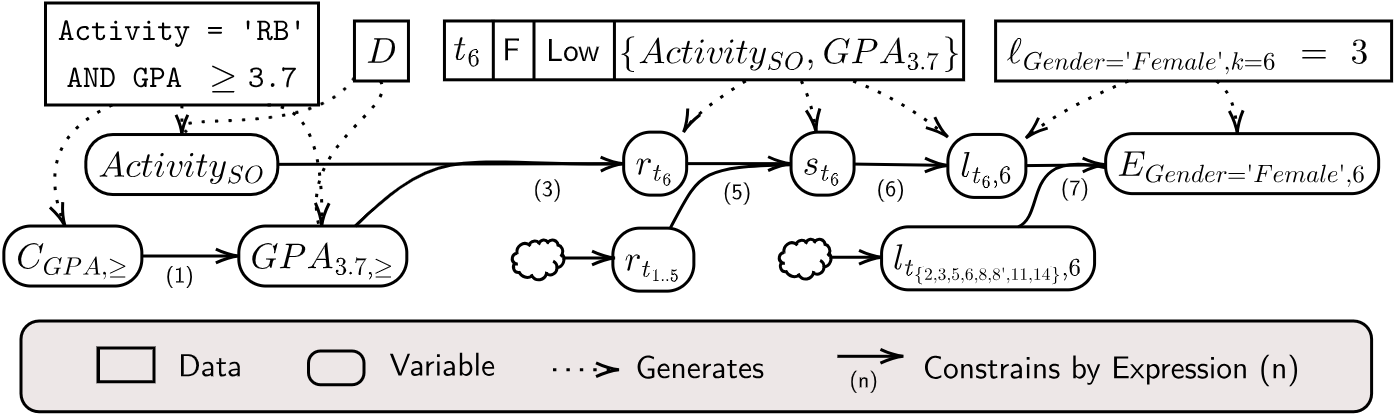
\includegraphics[width=\linewidth]{figures/example_summary.png}
    \caption{\revc{Diagram illustrating the expression generation for our running example. The predicate {\tt Activity = `RB' AND GPA $\geq$ 3.7} generates the variables $Activity_{SO}$ and $GPA_{3.7, \geq}$ as `SO' and $3.7$ are values that appear for those attributes respectively in the database $D$. $C_{GPA, \geq}$ is also generated by the predicate to hold the new constant of the predicate, and constrains the value of $GPA_{3.7, \geq}$ by (\ref{eq:value_bounds_inline}). The tuple $t_6\in \widetilde{Q}$ generates the variable $r_6$, whose value is constrained through (\ref{eq:tuple_in_ranking_inline}) by the values of $Activity_{SO}$ and $GPA_{3.7, \geq}$ due to its lineage. It also generates the variable $s_6$, which is then constrained by the value of the $r_t$ values for the tuples that rank better than it, i.e., $r_{t_{1..5}}$, through (\ref{eq:position_in_ranking_inline}). Finally, the constraint $\lb{Gender=`Female'}{k=6} = 3$ combines with $t_6$ to generate the variable $l_{t_{6},6}$ which is constrained by the value of $s_{t_6}$ by (\ref{eq:in_prefix_inline}). The constraint generates the variable $E_{Gender=`Female',6}$ which is constrained through (\ref{eq:tuples_to_satisfy_inline}) by the values of all the $l_{t, 6}$ variables for which $t$ is a part of the group (listed in \Cref{ex:deviation}).}}
    \label{fig:example_summary}
    \vspace{-0.5cm}
\end{figure}

%%%%%%%%%

% \subsection{Assignments}
% After constructing the instance of the MILP problem corresponding to the inputs of \problem{}, we use an existing MILP solver to produce an assignment $\alpha$ to the variables such that all expressions are satisfied. 
% % \yuval{Demonstrate using an example instead of the following. If possible, use the examples along the section}
% \begin{example}
%     \felix{splitting up}
    
%    % The variables $C_{Activity, RB} = 1$, $C_{Activity, SO} = 1$, $C_{GPA, \geq} = 3.7$ admit a feasible solution of our MILP model when refining the \running{} over the database shown in \Cref{ex:running}. Therefore, the set of constants for the refined predicate over $Activity$ is $\{RB, SO\}$. The refined constant of the lower-bound predicate on {\tt GPA} is then $C_{GPA, \geq}$, which is $3.7$. The refined query is finally
%    %  \begin{center}
%    %  \begin{small}
%    %  \begin{tabular}{l}
%    %      \verb"SELECT * "\\
%    %      \verb"FROM Students NATURAL JOIN Activities"\\
%    %      \verb"WHERE Gpa >= 3.7 AND (Activity = 'RB' OR Activity = 'SO')"\\
%    %      \verb"ORDER BY Sat DESC"\\
%    %  \end{tabular}
%    %  \end{small}
%    %  \end{center}
% \end{example}

%%%%%%%%%%%%%%%%%%%%%%%%%

\paragraph*{\revmulti{Model limitation}}
\label{sec:query_class_lims}
\revmulti{Given an input to our program, we construct a MILP program. The correctness of the solution generated by the program, as stated in \Cref{thm:bounded-deviation}, relies on three properties. First, every possible refinement may be represented as an assignment to the variables of the program. Second, the tuples in the output of any potential refinement are in the same relative order, and finally, every tuple in the output satisfies all the predicates of the corresponding refinement. We define the problem for SPJ queries, and thus, our model is designed to handle SPJ queries, and these properties hold for them. We note that supporting other classes of queries may require modifications to the problem definition as well as to our proposed model. For instance, in union queries, it is enough for a tuple in the output to satisfy the predicates of one branch of the union, in contrast to the third property. This may be handled straightforwardly, as noted in \Cref{sec:background}. Handling nested queries is more challenging since they may contain multiple selection statements at different nesting levels. The problem definition should first be extended to properly define how such a query can be refined, e.g., whether refinements at different nesting levels are allowed. Our proposed model cannot capture the refinement of selection statements in different nesting levels and, therefore, does not fulfill the first property. Moreover, if the {\tt ORDER BY} clause relates to an inner query, refining the inner query may change the relative order of the tuples in contrast to the second property.}


% In our presented model, these properties holds for SPJ queries but may be broken for other classes of queries. For instance, our model nested queries may not fulfill the first and second property as our model can not capture all possible refinements and


% It is important to note that the correctness of \Cref{thm:bounded-deviation} relies on some assumptions about the input query $Q$. We assume that $\widetilde{Q}$ is a query that retrieves all tuples that may be selected by any possible refinement, that the tuples in the output of any possible refinement are in the same relative order as in the output of $\widetilde{Q}$, and that a tuple fulfills all the predicates of the refinement. The first and second assumptions may be broken by a query that has subqueries: removing the predicates of the subquery and the parent query will not necessarily result in a query retrieving all possible tuples, and if the subquery is used as part of the {\tt ORDER BY} expression, refining it may change the relative order of tuples between refinements. The final assumption may be violated by a query with a union, where a tuple needs only to fulfill the predicates of one branch of the union. These assumptions are, however, fulfilled by SPJ queries, thereby motivating the limiting assumption made in \Cref{sec:background}. We note that our model may be extended to richer classes of queries if these assumptions are treated appropriately for these classes. 


% \paragraph*{\revmulti{Assumptions for correctness}}
% \label{sec:query_class_lims}
% \revmulti{It is important to note that the correctness of \Cref{thm:bounded-deviation} relies on some assumptions about the input query $Q$. We assume that $\widetilde{Q}$ is a query that retrieves all tuples that may be selected by any possible refinement, that the tuples in the output of any possible refinement are in the same relative order as in the output of $\widetilde{Q}$, and that a tuple fulfills all the predicates of the refinement. The first and second assumptions may be broken by a query that has subqueries: removing the predicates of the subquery and the parent query will not necessarily result in a query retrieving all possible tuples, and if the subquery is used as part of the {\tt ORDER BY} expression, refining it may change the relative order of tuples between refinements. The final assumption may be violated by a query with a union, where a tuple needs only to fulfill the predicates of one branch of the union. These assumptions are, however, fulfilled by SPJ queries, thereby motivating the limiting assumption made in \Cref{sec:background}. We note that our model may be extended to richer classes of queries if these assumptions are treated appropriately for these classes.} 

% \indent Recall that we obtain the lineage annotations for all tuples that may be returned by a possible refinement by evaluating $\widetilde{Q}$ over the database. However, consider a query $Q$ containing a subquery with selection predicates. Then, computing $\widetilde{Q}$ would not necessarily result in all the possible tuples. By removing the selection predicates from both the parent query and subquery, we get the set of tuples evaluated for that particular subquery rather than all the possible refined subqueries. Expression (\ref{eq:position_in_ranking_inline}) assumes that the relative orders between tuples are consistent between refinements in order to determine the position of the tuple in the output. If the subquery were used as part of the {\tt ORDER BY} clause, then it is possible that modifying the predicates of the subquery could change the relative order of the tuples between refinements. Expression (\ref{eq:tuple_in_ranking_inline}) assumes that a tuple must fulfill all the predicates of the query in order to be in its output. However, if $Q$ has a union such that $Q = Q_1 \cup Q_2$, then a tuple needs to only fulfill the predicates of (i.e. have its lineage included in) either $Q_1$ or $Q_2$.\\
% \indent These assumptions currently limit us to supporting SPJ queries, for which these assumptions are true: $\widetilde{Q}$ will return all possible tuples, the relative ordering of tuples between refinements remains consistent, and all predicates must be fulfilled in order for a tuple to be in the output. However, our approach is amenable to be extended to richer classes of queries, and in fact the extension to union is straightforward.}


%%%%%%%%%%%%%%%%%%%%%%%%%%%%%%%%%%%%%%%%%%%%%%%%%%%%%%

\section{Optimizations}
\label{sec:optimizations}
In Section~\ref{sec:search}, we have presented a MILP formulation designed to solve the \problem{} problem. While this approach enables us to leverage existing MILP solvers, that can solve the problem efficiently, they often encounter difficulties when dealing with extensive programs (containing numerous expressions), and a large number of variables~\cite{QFix}. While the number of expressions and variables in the MILP we generate is linear in the data size, as we show in Section~\ref{sec:experiments}, MILP solvers struggle to scale and solve the generated programs.


% , and struggle to scale (pointer to experiments). \yuval{can we say something about the number of expressions we generate?} 

To this end, we propose three optimizations for the construction of the MILP problem: one is a general optimization that applies in all cases, and the other two are limited in some cases. The first optimization is relevancy-based and removes from consideration tuples that are irrelevant to determining the satisfaction of the constraint set. The second optimization reduces the number of binary variables in the MILP problem by combining redundant variables. This optimization cannot be applied for queries with a {\tt DISTINCT} statement. %for queries without {\tt DISTINCT} statements.
The third optimization relaxes the expression used to determine the score of a tuple in the new ranking. This optimization is only applicable to tuples belonging to groups with only lower-bound or only upper-bound constraints, but not both.

%%%%%%%%%

\paragraph*{Relevancy-Based}
We propose a relevancy-based optimization to reduce the number of expressions and variables in our problem.
% to the mixed integer linear program in \Cref{fig:milp}, in order to reduce the number of expressions and variables in our problem. %It is noted in~\cite{QFix} that the performance of MILP solvers is in particular sensitive to these parameters. 
Recall that we use $k^*$ to denote the maximal $k$ that appears in the constraint set $\constraints$. Then, by removing tuples that could never appear in the top-$k^*$ in any refinement, we are able to avoid adding their variables and expressions to our problem. We determine the relevancy of these tuples by selecting the top-$k^*$ of the groups of tuples that share the same lineage. Let $[\prov(t)]$ be the equivalence class of tuples that share the same lineage as a tuple $t$. Then for a tuple $t$, let $T(t)$ be the ranking generated by ranking the tuples of $[\prov(t)]$ according to the {\tt ORDER BY} clause of $Q$. We see trivially that it is not possible for tuples past position $k^*$ in $T(t)$ for all $t$ in $\widetilde{Q}(D)$ to be included in the top-$k^*$ of any refinement. Thus, it is sufficient to consider only the top-$k^*$ of $T(t)$, denoted by $T(t)_{k^*}$, in the generated program, and we replace $\widetilde{Q}(D)$ in the expressions referencing it with $T(t)_{k^*}$ in Figure~\ref{fig:milp}. 


% We then substitute $\widetilde{Q}(D)$ in the expressions referencing it with the ranking generated by $\bigcup_{t \in \widetilde{Q}(D)} T(t)_{k^*}$ ranked according to the {\tt ORDER BY} of $Q$.

% \indent We define $k^*$ as the length of the maximal prefix of the constraint set $\constraints$. Then, by removing tuples that could never appear in the top-$k^*$ in any refinement, we are able to avoid adding their variables and inequalities to our problem. We determine the relevancy of these tuples by selecting the top-$k^*$ of the groups of tuples that share the same lineage. Let $[\prov(t)]$ be the equivalence class of tuples that share the same lineage as a tuple $t$. Then, let $T$ be the ranking of $[\prov(t)]$ according to the {\tt ORDER BY} clause of $Q$. We see trivially that it is not possible for tuples past position $k^*$ in $T$ to be included in the top-$k^*$ of any refinement. We then substitute $\widetilde{Q}(D)$ with $\bigcup_{t \in \widetilde{Q}(D)} T_{k^*}$ ranked according to the {\tt ORDER BY} of $Q$ in all definitions of our inequalities.
\begin{example}\label{ex:optimization1}
    % Continuing from our running example, consider the tuple $t_{14}$ with $\prov(t_{14}) = \{Activity_{RB}, GPA_{3.7}\}$.
    %\yuval{The lineage is defined with respect to the query. This is not the lineage of the tuple in the running example}. 
    Consider $t_{14}$ from Table~\ref{tab:joined}. Its equivalence class $[\prov(t_{14})]$ is the set $\{t_7, t_{10}, t_{14}\}$. Assume we are interested in satisfying a single constraint $\lb{Gender=`Female'}{2} = 1$. Note that the tuple $t_{14}$ can never appear in the top-$2$ of any refinement query, as any refinement that includes $t_{14}$ includes tuples with its same lineage, i.e., $t_7$ and $t_{10}$. Therefore, it is safe to remove all variables and expressions related to $t_{14}$ from consideration.
    % Then, the equivalence class $[\prov(t_{14})]$ is the set $\{t_7, t_{10}, t_{14}\}$. For simplicity, consider instead a singleton constraint set with a smaller maximum prefix: $\lb{Gender=`Female'}{2} = 1$. The deviation from the constraint then depends only on the top $2$ tuples. Now, notice that the tuple $t_{14}$ may never appear in the top-2, as any refinement that includes $t_{14}$ includes tuples with its same lineage, i.e., $t_7$ and $t_{10}$. The tuples $t_7$ and $t_{10}$ rank better than $t_{14}$, meaning that $t_{14}$ can never be in the top-$2$. Therefore, it is safe to remove $t_{14}$ from consideration. 
\end{example}
This optimization is most effective when $k^*$ is small, and there are few lineage equivalence classes. In \Cref{sec:experiments}, we show that this is often the case in queries over real data sets. We further demonstrate the effect of $k^*$ on the running time in \Cref{fig:time_vs_k}.

% this in \Cref{fig:time_vs_k}, which shows that the running time of the algorithm increases with $k^*$.

%%%%%%%%%

\paragraph*{Selecting Lineages} 
% The next optimization leverages the notion of lineage equivalence classes to reduce the number of variables. 
Recall that the program we generate includes a binary variable $r_t$ for each tuple in $\widetilde{Q}(D)$. However, tuples sharing the same lineage all have equal values for their $r_t$ variables. Therefore, we can use a single variable for all tuples in the same lineage equivalence classes. 

% The idea is to use a single variable for all tuples with the same lineage instead of their $r_t$ variables, as they all share the same assignment. 
% We propose another optimization to reduce the number of variables constructed in the MILP problem by using this notion of lineage equivalence classes to select all the tuples of a selected lineage with one variable, instead of constructing variables for tuples individually. \\
% \indent Our original construction of the MILP problem creates a binary variable $r_t$ for each tuple in $\widetilde{Q}(D)$. However, tuples sharing the same lineage all have equal values for their $r_t$ variables. Therefore, many of these variables are redundant and could share one variable made for the tuples of its lineage instead.
\begin{example}
    To demonstrate this idea, consider the \running{} without its {\tt DISTINCT} statement and consider again the tuple $t_{14}$ with its equivalence class shown in Example~\ref{ex:optimization1}. If $t_{14}$ satisfies the selection condition of a refinement on the \running{}, then $t_7$ and $t_{10}$ must satisfy the conditions as well, as they share the same lineage. Therefore, we have the equivalence $r_{t_{14}} = r_{t_7} = r_{t_{10}}$. The variables $r_{t_7}$ and $r_{t_{10}}$ are then made redundant, as they always have the same value as $r_{t_{14}}$. 
\end{example}

In order to avoid such redundancy, instead of constructing the set of $r_t$ variables, we construct a set of variables $r_{[\prov(t)]}$ for every tuple $t$ in $\widetilde{Q}(D)$. Using (\ref{eq:tuple_in_ranking_inline}) as a basis, we are able to model $r_{[\prov(t)]}$ being assigned $1$ if and only if the tuples in $[\prov(t)]$ satisfy the selection condition of the corresponding refinement query.
% the lineage is selected.
 Instead of constructing expression (\ref{eq:tuple_in_ranking_inline}) for each tuple in $\widetilde{Q}(D)$, we construct the following expression for each $r_{[\prov(t)]}$ variable:
% \begin{align*}
    $0 \leq \sum_{p \in \prov(t)} p - |\conds(Q)| \cdot r_{[\prov(t)]} \leq |\conds(Q)| - 1$.
% \end{align*}
Furthermore, in order to ensure that the $s_t$ values are modeled as before, we modify (\ref{eq:position_in_ranking_inline}) by changing $r_t$ to $r_{[\prov(t)]}$ and $r_{t'}$ to $r_{[\prov(t')]}$.
We note that this optimization cannot be applied if the input query includes a {\tt DISTINCT} statement,
% However, we cannot use this optimization where the input query has a {\tt DISTINCT} statement,
as we need this information in order to not select tuples that already have a tuple sharing its distinct value selected.
%%%%%%%%%

\begin{table*}[t!]
    \centering
    \footnotesize  
    % \hspace*{-0.5cm}
    \begin{tabular}{lclcl}
    \hline
    \textbf{Dataset} & \textbf{Query} & \multicolumn{1}{c}{\textbf{Predicates}} & \textbf{Order by (DESC)} & \multicolumn{1}{c}{\textbf{Constraints}}\\ \hline\hline
    Astronauts & $Q_A$ & 
    \begin{tabular}{l@{}}\texttt{"Graduate Major" = 'Physics'}\\ \texttt{AND "Space Walks" <= 3}\\ \texttt{AND "Space Walks" >= 1} \end{tabular}  
    &{\tt "Space Flight (hrs)"}&\begin{tabular}{@{}ll@{}}
        (1) $\lb{Gender='F'}{k} = \frac{k}{2}$ & (4) $\lb{Status='Management'}{k} = \frac{k}{5}$ \\ (2) $\lb{Gender='M'}{k} = \frac{k}{2}$ & (5) $\lb{Status='Retired'}{k} = \frac{k}{5}$ \\ (3) $\lb{Status='Active'}{k} = \frac{k}{5}$ &
    \end{tabular}\\
    \hline
    Law Students & $Q_L$ & \begin{tabular}{l@{}}\texttt{Region = 'GL'}\\\texttt{AND GPA <= 4.0}\\\texttt{AND GPA >= 3.5}\end{tabular}& {\tt LSAT}&\begin{tabular}{@{}ll@{}}
        (1) $\lb{Sex='F'}{k} = \frac{k}{2}$ & (4) $\lb{Race='White'}{k} = \frac{k}{5}$ \\ (2) $\lb{Sex='M'}{k} = \frac{k}{2}$ & (5) $\lb{Race='Asian'}{k} = \frac{k}{5}$ \\ (3) $\lb{Race='Black'}{k} = \frac{k}{5}$ &
    \end{tabular}\\
   \hline
    MEPS & $Q_M$ & \begin{tabular}{l@{}}\texttt{Age > 22}\\\texttt{AND "Family Size" >= 4}\end{tabular}& {\tt Utilization}&\begin{tabular}{@{}ll@{}}
        (1) $\lb{Sex='F'}{k} = \frac{k}{2}$ & (4) $\lb{Race='Black'}{k} = \frac{k}{5}$ \\ (2) $\lb{Sex='M'}{k} = \frac{k}{2}$ & (5) $\lb{Race='White'}{k} = \frac{k}{5}$ \\ (3) $\lb{Race='Asian'}{k} = \frac{k}{5}$ &
    \end{tabular}\\ \hline
    TPC-H & $Q_5$ & \texttt{Region = 'ASIA'} & {\tt Revenue}& \begin{tabular}{@{}ll@{}}
        (1) $\lb{OrderPrio='5-LOW'}{k} = \frac{k}{2}$ & (4) $\lb{MktSeg='BUILDING'}{k} = \frac{k}{5}$ \\ (2) $\lb{OrderPrio='3-MEDIUM'}{k} = \frac{k}{5}$ & (5) $\lb{MktSeg='MACHINERY'}{k} = \frac{k}{5}$ \\ (3) $\lb{MktSeg='AUTOMOBILE'}{k} = \frac{k}{5}$ &
    \end{tabular}\\ \hline
    \end{tabular}
    \caption{Queries and constraints}
    \label{tab:queriesAndConstraints}
    \vspace{-0.5cm}
\end{table*}

\paragraph*{Relaxation for Single-Constraint-Type Tuples}
%\yuval{this part is still not clear}
We present another optimization that is possible when a tuple belongs to groups that have only either lower-bound ($\ell$) or upper-bound ($\mathscr{u}$) cardinality constraints made on them. We define the set of tuples belonging only to groups with lower-bound constraints as 
% $$L = \{ t \mid \not\exists (\ub{G, k} = n) \in \constraints, t \in \sigma_G(\widetilde{Q}(D)) \}$$
$L = \{ t \mid \not\exists (\ub{G}{k} = n) \in \constraints, t \in \widetilde{Q}(D) \cap G \}$.
We define a similar set $U$ for upper-bound tuples, replacing $\ub{G}{k} = n$ in the quantifier with $\lb{G}{k} = n$. Then, for a tuple $t \in L$, we relax expression (\ref{eq:position_in_ranking_inline}) to 
$1 + |\widetilde{Q}(D)| \cdot (1 - r_t) + \sum_{t' \in \widetilde{Q}(D), \widetilde{Q}(D)(t') < \widetilde{Q}(D)(t)} r_{t'} \leq s_{t}$.
% We may relax tuples in $U$ similarly by specifying an upper bound instead. 

For tuples in $U$ we use an upper bound instead ($\geq s_t$). This relaxation makes finding feasible solutions for this model easier and may be used by presolving techniques in MILP solvers.
% 
To understand why this maintains the correctness of our solution, consider the lower-bound constraints. Intuitively, we can allow the $s_t$ variables of tuples belonging to the group defined in the constraint in a given top-$k$ to be assigned a value larger than the position of $t$ in the ranking, as this can only result in a worse deviation from satisfying the constraint (but can not assign a value smaller than the position of $t$ in the ranking). The case for upper-bound constraints is symmetric.




% "leave" it (i.e. assign $s_t$ a value larger than the position of $t$ in the ranking), as this can only result in a worse deviation from satisfying the constraint. However, we cannot have the tuples belonging to this group outside of that prefix "enter" it (i.e. assign $s_t$ a value smaller than the position of $t$ in the ranking), as this might result in claiming a lower deviation than reality. The case for upper-bound constraints is symmetric.

% \begin{example}
%     Consider the assignment feasible for (\ref{eq:value_bounds_inline}-\ref{eq:position_in_ranking_inline}) corresponding to the original \running{}. Let $t_{14}$ be the tuple corresponding to student \#14 in \Cref{tab:candidates} joined with \Cref{tab:internships} (shown in \Cref{tab:joined}). In the ranking $R$ generated by the query, we have $R(t_{14}) = 7$. Therefore, we have $s_{t_{14}} = 7$. However, by making the relaxation as seen above, we instead have $s_{t_{14}} \geq 7$, meaning that this tuple can not be used to count towards satisfying the cardinality constraint $\lb{Gender='Female'}{6} = 3$.
% \end{example}